\chapter{Experimental investigations}

For understanding and analysing double descent and bias-variance trade-off, and furthermore in later section on identifying double descent, we would like to use test models specifically for exhibiting bias-variance, as well as testing hypothesis and forming theoretical conjectures. This is because of the troublesome nature of the phenomena itself, which proves difficult to analyse without sufficient experimental observations. Furthermore, specific analysis on these types of model might prove useful for generalization toward more difficult and complex structure. 

Our major focus is on three types of model. First two are classical models and system, linear models on the real space $\mathbb{R}^{n}\to\mathbb{R}$. Second, is the type of \textbf{support vector machine} (SVM) models to highlight the analysis toward data-based fundamental analysis. The third one is the class and collection of different \textit{neural network structures} (MLP, or variations). Our goal is then to expansively analyse, formalize, making conjectures and hypothesis and test them, to find, force double descent out, or identify it on the learning landscape. We note that structures of those models are not well-generalized, hence analysis from one might not apply or apply only in small conjunction. This approach is rather quite helpful in its own merit, as its choice and preference will gauge our parameters than we gauge the phenomena of the parameter it induces.
\section{Experimental planning}

This section of the manuscript will explicitly contain instructions, setup, methodology, and so on, with regard to the experimental details of the experiments itself. In all, we would be covering the scheme of optimization algorithm responsible for dynamical modelling, and the other one for one-shot analytical optimization of the least-square form. Furthermore, justification and experimental list, with detailed analysis of each case of the system in consideration of testing would be included so much so to condition the test on the ground of generality as far as possible, and proliferate the experiment coverages. We also cover interpretation, and dataset generation, if such would be elucidated, and the concept of \textbf{stress-testing} under formal experimental package, if such is included in later analysis. 

\subsection{Setting: gradient-based optimization}

In our usual experiment, we would most specifically, use a closely-regarded family of gradient-based algorithms, such as gradient descent (\cite{Cauchy:1847,Robbins:1951,Widrow:1960,Hestenes:1952,Fletcher:1964}), mirror descent, natural descent, and so on (\cite{nemirovski_yudin_1983,amari_1996_natural_riemannian_gradient,amari_1998_natural_gradient_works,yang_amari_1998_complexity_issues_natural_gradient,amari_rattray_saad_1998_natural_gradient_online,gunasekar_woodworth_srebro_2021_mirrorless_mirror_descent,luong_parpas_rueckert_rustem_2016_weighted_mirror_descent,xiao_zhang_2014_proximal_stochastic_gradient,sohl-dickstein_2012_natural_gradient_whitening,raskutti_mukherjee_2013_information_geometry_mirror_descent}). While implementation and details of the specific algorithm can be different, they all shares some of the same concepts of which making them possible for optimization in the specified iterative domain. The most general formulation possible is the following algorithm on convexity of the gradient descent family. 
\RestyleAlgo{ruled}
\SetKwComment{Comment}{}{}
\begin{algorithm}[htb]
    \caption{Gradient descent on general (convex) function}
    \KwData{$(x_{i},y_{i})\in\mathcal{S}$, $\eta$, $\nabla(\cdot)$ operator, hypothesis model $h\in\mathcal{H}$, arbitrary construction on complexity $d$.}
    \KwResult{Expected optimization to the minimal error on $\ell(\cdot,\cdot)$.}
    \Begin
    {
    $\mathbf{w}\gets$ randomly initialized values on operation\;
    $\mathbf{w}_{1}\gets$ first \textbf{state} of the state space $\mathbb{W}\subseteq \mathbb{F}^{q}$ for $q$ specified by $d$ complexity.\;
    \For{$t\gets 1$ to $T$}{
        $\mathbf{y}\gets \{h(\mathbf{x})\}^{|\mathcal{S}|}$\;
        $\mathbf{w}_{t+1}\gets w_{t}\odot\eta\nabla_{\mathbf{w}} M_{\ell}(h[\mathbf{w}](x))$, arbitrary $\odot\equiv (-)$ under normal operator, loss evaluation configuration $M_{\ell}$. 
    }
    }
    \Return{Model $h[\mathbf{w}_{T}](x)$ such that $\displaystyle{\argmin_{\mathbf{w}\in\mathbb{W},h\in\mathcal{H}} M_{\ell}(h[\mathbf{w}](x))=h[\mathbf{w}_{T}](x)}$.}
    \label{algo:algo_gd}
\end{algorithm}

Specifically, the scaffolding of the gradient descent algorithm is on the encoding of all numerical entities - we presuppose as the framework a form $h(x)$ fixed functional composition, such that the space $\mathcal{H}$ is a function space of all admisible descriptions on $[qh_{1},\dots,qh_{n}]$ of the hypothesis element construction, such space $\mathcal{H}$ incurs $h(x)$ with its parameters form $\bm{\theta}$ or $\mathbf{w}$ (depends on notation) of sort in compressed notation, hence the model lives in a flat parameter initialization, typically can be compressed to 1-D slice value representation. Often time, we have the parameter or any form of structural descriptions of a model without the second pair on composition and operations $\Gamma_{h}$ to live on the \textbf{state space} $\mathbb{W}$, but on presentation status, we can reduce it to repeatable many-point domain. Adding the second dimension on the space to be the conjunctive $(y,y_{h})$-domain, we have the now applied $[\mathbf{w},\mathbf{y}]$-space. For grounding, the last representation contains $\mathbf{x}$ for the numerical setting that are inputs to both. In all, we have a 3D space on $[\mathbf{x},(\mathbf{y},\mathbf{y}'),\mathbf{w}]$, of which can be used to experiment and observe different tracing of paths. 


Nevertheless, one should be cautioned of the intrinsic assumption on which gradient descent of this type assumes. It assumes \textit{convexity}, which can only be possible, if the landscape itself is supposedly, assumed to contain such global minima. Said global minima in a richer language can be described as the epistemic collapse of the learning structure, under the arbitrary optimization space. This is a \textit{very serious assumption}, and should it fail, as seen in a lot of non-populated or general observation space, the entire procedure is invalid. It is also troublesome as to rely on the singular objective (numerically encoded) space in which it is trivial to realise that there are indeed, local minima. This scaling, with respect to both locality and global consideration, must be considered carefully, since \textit{every single contribution} might distort the experiment in a very unexpected way. In a more sophisticated explanation, we would be more aware of the structural conformation that gradient descent make of the encoding space. If one wish, the formulation can be changed to 
\begin{equation}
    \argmin_{\epsilon\geq 0;\:\mathbf{w}\in\mathbb{W},h\in\mathcal{H}} M_{\ell}(h[\mathbf{w}](x))=h[\mathbf{w}_{T}](x)
\end{equation}
for the arbitrary condition of $\epsilon$-fitness, which relaxes the argument. However, it introduces the determination value of $\epsilon$, whether such is achievable or not which means the algorithm requires \textbf{termination mode}, which lies in the hand of computability design, and how $\epsilon$ behaves and specific instance of forcing on such direction. 
\subsection{Experiments list}

The following describes and outline specific requirements updated of experiments, aside from done experiments. Currently, there remains the \textit{neural network} in plain form functional approximator experiment, \textit{polynomial neural network (customized)} experiments, validation of \textit{support vector machine (SVM)} on generalized task space experiments, different large-scale neural networks (VGG, ResNET, LLM) experiments set, and toy model for investigations. Specifically:

\begin{enumerate}[itemsep=1pt,topsep=1pt]
    \item \textbf{Linear models on abstract $\mathbb{R}$-conjunction space\footnote{Conjunction space simply means that the full numerical encoding space of all activities involved}}: Different kind of components-based on linear behaviours, in different setting and so on, of different testing scenario (regression, classification). 
\noindent Linear model are often the canonical example of double descent, as they offer a rather simplified setting that most often would be tractible for analysis. Thereby, we will start with experiments and surveillance of different settings under such spaces, and actual implementation and testing rigorously thereof for linear regression. 

    \item \textbf{Polynomial-type models on abstract conjunction space}: Similar to the above linear case, this one however allow for polynomial-style components, i.e. degree $k$ terms up to $n$th degree. 
    \item \textbf{Support Vector Machine (SVM) on abstract spaces and sample space}: The SVM model is rather interesting (within which it has regression and classification as main functionality), because it goes reverse from perspective - instead of creating models to fit data, it uses data to create fitting model. 
    \item \textbf{Neural network on-layer, abstract functional spaces}: This is the set of experiments for layer-based neural networks, on abstract functional spaces of analysis. The list includes vanilla $(l,n)$-mass neural network with mixed activation patterns, CNN, VGG, ResNet, spatial neural networks, RNN, LSTM, and if able, certain precursor of LLM systems. 
\end{enumerate}

All of those models base their purposes in \textit{component-based interpretation}, such that the scope in which their components are allowed, change the dynamics and so on of the model. The theoretical problem of which those experiments are targeted on is to mark the singular hindsight - \textit{simply how} model behaves under controlled structural changes and setting changes. Because of the lacking in such deference of approaches, it also depends heavily on how the adversarial set (dataset, concept) itself is targeted of, or coverage of such. Such is to say, we also need the \textit{precursor theory} of component treatments. Which is explained above, but such is also particularly extensible to explain also grokking (\cite{Power2022Grokking,Liu2023GrokkingExplained}), benign overfitting (\cite{Bartlett2020BenignOverfitting,Muthukumar2021Interpolation}), \textit{neural collapse} (\cite{Papyan2020NeuralCollapse,Han2022NeuralCollapseSurvey}), optimization-based anomaly or phase-transition similar form (\cite{Cohen2021EdgeOfStability,Fort2019DeepLossLandscape}), and the fuzzy, diverged front of explanations in deep learning phenomena, as criticized by \cite{Razeghi2025ExplanationCritique}. 

\subsubsection{A note on polynomial neural networks}

Because of the sensitive context of double descent, polynomial suffers the same fate of design, as so is many of the experiments. Its design implementation details must be explicit. That is, of which can be seen in the polynomial transition model. That said, the setting itself is rather more difficult to assess. 

Originally, it is asked of the experimental team to set up \textbf{adversarial testing}, i.e. testing two mismatched polynomial models together, in a singular testing system. So, we will have $(p_{k},p_{c})$ for $k\in[a,b]$ of complexity specification, in this case, the number of initialized degree of interest. As such, the experimental system is between two polynomials. But this turns out to have certain problem: \textit{domain range}. The domain value, when admitted of the input $x\in\mathbb{R}$ or $\mathbf{x}\in\mathbb{R}^{n}$ of $n$-dimensional input sequence, is rather difficult to control, especially for $[a,b]$ that is nonstandard in $[-1,1]$, and not of normalized unit. Usually, we understand the polynomial transition space as the modular $\mathbb{R}\to\mathbb{R}^{h}\to\mathbb{R}$ mapping for singular $n$-dimensional hidden field, the polynomial basis terms. However, if we are to upgrade it to multivariate polynomial, such changes dramatically, and so is the structure itself. Thereby, so is the behaviours on ranges. The justification for nonstandard, free monomial is that for increased value range, the pattern is not chaotic, but rather smoothed out by dominant terms, for example, the $n$-degree terms contribution in univariate case. Similar case happens when taken into consideration $n$-dimensional polynomial mapping on $\mathbb{R}^{n}\to\mathbb{R}^{m}$, but only this time the dominance is local to individual dimension itself. In general,

\begin{conjecture}
    The probability of dataset representing wrong $n$-univariate polynomial $p_{n}$, on finite arbitrary space $\mathcal{D}=[a,b]$, for $|\mathcal{D}|\to\infty$, increases, in presence of $\epsilon\sim\mathcal{N}(a,\sigma)$ noise. 
\end{conjecture}

The main fundamental reason is because of the ill-conditioned Vandermonde basis, in which is typically used in polynomial expression. Elsewhere, on finite space $[a,b]_{m}$ on $m$ samples, it is then conjectured that the chance of interpolation is much greater, and much more deviated from the actual concept shape if stray over large enough $[a,b]$, thus also influence the error rate and gradient-based learning form of different weights. The goal is then, to construct rich enough polynomial concept class, based in this new discrete, finite range and initialization goals, with the main goal is to find sufficient polynomial construction on arbitrary $[a,b]\in\mathbb{R}$ that $y$ foes not explode. This is fundamentally hard, and if unable to procure, we would have to choose to go for the normalized space on $[-1,1]$. This is also for computational purpose, since \texttt{float128}, of which is the main data point form, is numerically unstable with large operations and the density of operations as such without sufficient safety control, in which it is very hard to reconcile. 

One more point to note. What we have seen is based on the perception of typical machine learning setting that \textbf{monomial Vandermonde basis} is the polynomial representation space. In fact, this is not true, as there are many as Lagrange polynomial, Newtonian basis, Legendre polynomials, and different classes of orthogonal polynomials. However, without structural operational analysis, such addition and generalization is hard to tract of the structural droplet they introduce. 

The following will list the amount or configuration that test should be taken into consideration, first with the guideline. 

\begin{enumerate}[topsep=1pt,itemsep=1pt]
    \item \textbf{Carefulness on numerical processing}: Introducing polynomial models meaning that for each component, it is reducibly equivalent to $n$ linear components, for each component, with multiplicative combinator. So for example, a system of full $n$-degree model sequentially, would have $n!+1$ linear equivalent mass size, including the bias on numerical space. Therefore, the value in practical calculation can be very large, even in $[-1,1]$ as the pairwise normalized. Cares then must be taken to draw that out. 
    \item \textbf{Minimal implementation}: Use the least, but consistent code possible. Each code must be recommended to be designed modularly, such that you can snap it in others with only relevant knowledge as to \textit{what it does} and \textit{what is the typing allowed} of the unit itself, aside from utility systems. 
    \item \textbf{Loop collapse}: The order of loop, or changing test case is very necessary to be taken into account of. First one, is the \textbf{system test loop}, where the setting of the environment for operation, i.e. noise, concept allowed (dimension or description or class of types), number of samples, and so on. The second one is the \textbf{hypothesis-action loop}, of the empirical action of \textit{train-test-validate-cross} partition of the observational space $\mathcal{S}_{n}$ to mimic generalization in oracle setting, the hypothesis spaces, and so on. The final one is the \textbf{operational level}, where you specify the loss-landscape, learning metric, aggregated measures, loss function measure, actions on learning algorithms, the learning algorithm configurations (for example, learning rate, etc.), and so on. 
\end{enumerate}
Aside from such, each layer in the final point \textit{procure measures and statistics}. For example, at system test loop, you have properties of the dataset itself. Distribution and shape or form of the model as the second loop, and so is the jump path, approaches, pathology of the reconstructed loss space. Such should be taken into consideration. The list of model is then:

\begin{enumerate}[topsep=1pt,itemsep=1pt]
    \item Polynomials, function concept set: This is where we do not require the setting of two-polynomial model configuration together and to study them using a class of different elementary function, only fit the input-output space. For example, singular $sin(\cdot)$ class that fits $\mathbb{R}\to\mathbb{R}$ is ideal, or else, or different pathological systems. 
    \item Polynomial, adversarial $[-1,1]$ range: Construct both, only in $[-1,1]$ range for evaluation, since higher range collapses into smoother values. 
    \item Polynomial, changing basis construction, $[-1,1]$ range: Use modules, like \texttt{numpy.polynomial.legendre}, or \texttt{scipy.special.legendre}, and so on. 
    \item Polynomial, changing basis (plus monomial), $[-1,1]$ range, input-dropout (filter): Filter out, in the form of hidden information from the hypothesis polynomial, and not the concept polynomial, to simulate ordered information mismatch. 
\end{enumerate}
One of the main examples would be to pitch different kind of models together, for example, targeting Legendre polynomial class on monomial going against Newtonian polynomials, or the Vandermonde basis going against other structural models as well. On the reduction of range, what we have done are conditioning upon the instability of large numerical values. This is only a temporary solution, and would almost change the geometry of the problem significantly. As such, methods aside from such mapping reductio can be suggested instead of flat collapse. Several choices are possible, including \textit{affine normalization}, $x'=(x-\mu)/s$ for $\mu$ as the centre of the arbitrary range $[a,b]$ that was previously presented, and $s$ as the characteristic custom scale parameter. The cost incurred here is reversible on affine transformation, preserving domain semantics. Standardization or z-score on $x'=(x-\bar{x})/\sigma$ rescaling, whitening (PCA) on $x'=\Lambda^{-1/2}U^{\top}(x-\bar{x})$ from SVD of the covariance on the dataset structure, Log/Box-Cox transformation, and many more to be specific. In the following up deployment of learning presentation, we would like to examine its behaviour on such space. 

\subsection{Preliminaries on observations - \cite{schaeffer_double_2023}}

Conveniently, one of the few analytical sufficient experimental analysis that we can get, is from \cite{schaeffer_double_2023} paper on demystifying double descent. While the experimental setup is rather well-defined and interesting, it is also rather limited in scope, of which we want to dive deeper into it and further the analysis that was provided. The setting of the model in precondition was within the setup of a duplet correlation dataset, 
\begin{equation}
    \mathcal{D} = \{(\mathbf{x}_{n}, y_{n})\}_{1\leq n \leq N}
\end{equation}
for $N$ samples with variational vector $x$ as input. The function is the classical functional type of $y=c(\mathbf{x})$ of the hidden concept, of which is assumed to utilize all variables in the setting of $\mathbf{x}$ itself. Thence, objective is to figure out for the model $f(x)$ given, such that
\begin{equation}
    f(\mathbf{x}) = \mathbf{x}\cdot \bm{\beta} \approx c(\mathbf{x}) 
\end{equation}
In a sense, if the setting is ordinary linear regression, then such model equates to multilinear model, unless $|\mathbf{x}|=1$, without bias $b$ on the conditioned projection space. The experiment conducted in the test is rather simple, with the setting being,
\begin{equation}
    |\mathbf{x}| = 1,\quad x\in [-1,1],\quad y\in \mathbb{R},\: c(x) = 2x + \cos{(25x)}
\end{equation}
and within such approximating $c(x)$ using a univariate polynomial on feature map $\bm{\phi}_{P}$ of which maps any $x$ to $P$-degree polynomial basis vector, and collapse it of such for the fitting model $f(x)$ to be now
\begin{equation}
    f(x)\equiv \bm{\phi}_{P}(x)\cdot \beta_{P} \approx c(x)
\end{equation}
While the paper indeed introduced a larger and logical intuition concepts, plus analysis into how one might interpret such result using ordinary least square and the general regression problem, such is often poorly directed toward where the analysis itself is rather only additive than any. First, is the legible assumption of the generality of application on results, of the tested function class of cosine class functions with additive conditional bias drift on $2x$ term. The paper insufficiently so, does not tell us about how this visual explanation and analysis can help us in understand more about double descent aside from the optimization path analysis already did in several other analyses. The family of cosine equations itself imposes a rather non-trivial properties, it forces \textbf{periodicity} and value space bounding on dataset itself. That is, the choice of giving cosine class concept function morphs the moving optimization space to a more narrow space, on which there exists $x$-consistent spread and structures, i.e. a \textbf{concentrated space} class. During which, the shift can give the cosine class a linear upward drift, but not enough toward which to be called exploding, like in many cases of polynomial models or complex pollinated classes dynamics. Effectively, such is to constrain $c$ into the real analytic on compact interval problem, or $c\in C^{\omega}([-1,1])$ space, and of which spectral decays and heavy-tailed or sparse spectral structures are rare or nonexistent. 
Second, constraining the setup to $[-1,1]$ directly interferes with the stability of the ill-conditioned Vandermonde basis polynomial space, of which setup a rather non-trivial optimization path under iterative algorithms. Thirdly, the experiment deliberately removes noise-conditioning setting, of which means that the setting assume of the synthetic analysis \textit{full oracle access} on details, of which is a non-trivial choice. 

Continuing forward, the three critical quantities are generally rather not explained. For example, it is mentioned that removing small singular values in the training features $X$ prevents double descent, however such removal is non-trivial and requires justification on why this is a rather good choice, and whether a synthetic dataset can remove such and \textit{where} would it be so. Preventing the test feature from varying in trailing singular modes prevents double descent, however with such singlar modes are there is unknown, and there are no justification - whether if such mode is detrimental to the actual dataset or not of the arbitrary concept classes. Similarly so, ensuring that the optimal model in the model class has zero residual prediction errors $E$ is stated to prevent double descent, however, that is a rather metric-dependent optimization scheme, and might as well lead to the \textit{overfitting regime}, where at this behaviour, one actually returns to the question of overfitting both test and train sets, and would have to rely on the third set to see if double descent appears there or not. Either way, the setting itself is interesting to analyse, and one would consider it interesting to expand on their analysis, especially to different finite-domain conditioned system and concepts. 

\section{Data generation}

Dataset generation, coming off the analysis on the actual complexity of the concept, structural exchanges and thereof, requires at this stage deliberate elaboration on the method of synthesizing. Indeed, while typical dataset on synthesizer are often obtained by hard-coded artefact, plus random noise $\epsilon\sim\mathcal{N}(0,1)$, such is rather not desirable and certainly not the only type of noise in the toolbox of statistical analysis. Certainly so, this is illustrated in Figure~\ref{fig:generative_dataset_condition_1}, where there exists a rather rich family of noise to consider, that perhaps are non-trivial of analysis given the fact that different noise profile can be either irreducible, or by virtue contains structural details hidden from what we observed of the relationship itself. 
\begin{figure}[htb]
    \centering
    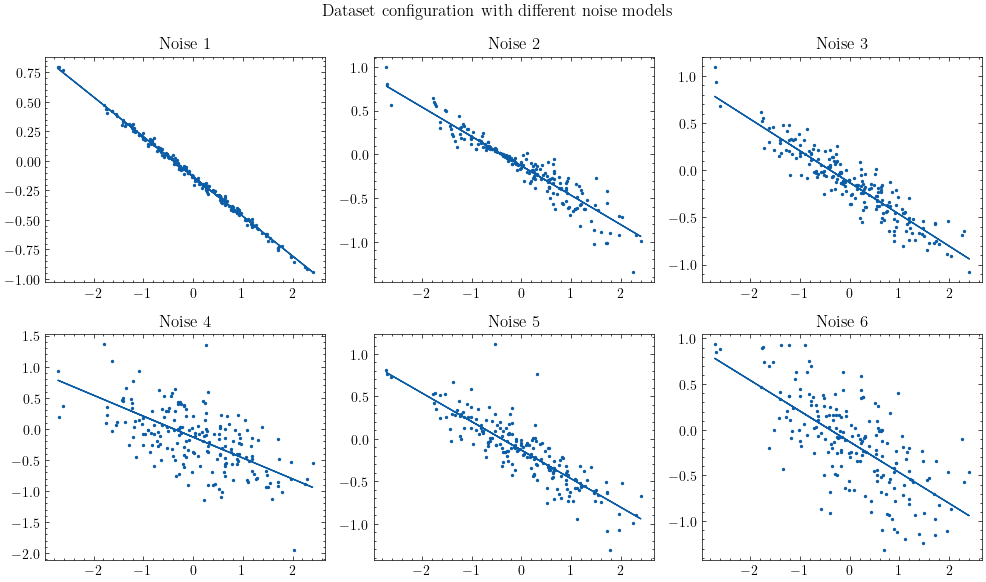
\includegraphics[width=0.8\textwidth]{img/generation_condition_1.png}
    \caption{The different variations of the noise profile that can be often seen when sampling from a simple regression model. By order, (1) represents mean-scale additive noise, (2) considers heteroskedastic multiplicative noise, (3) considers variance-scaled additive noise, (4) considers absolute additive noise (where scale independent of $y$), (5) considers heavy-tailed noise (Student-$t$ modelling), and (6) is the standard canonical Gaussian noise (basically the default). All are under reduced dimension of the simplest linear model on feature space as possible for illustration.}
    \label{fig:generative_dataset_condition_1}
\end{figure}
\begin{figure}[htb]
    \centering
    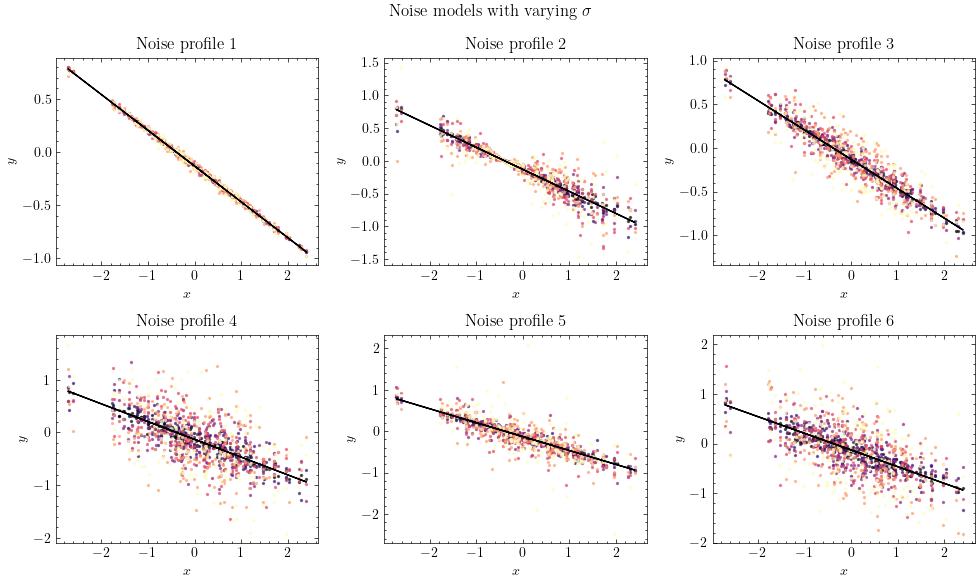
\includegraphics[width=0.8\textwidth]{img/generation_condition_2.png}
    \caption{The different variations of the noise profile that can be often seen when sampling from a simple regression model, but for different controlling nob for strength of the noise, by $\sigma$ in range of $[0.1,0.2,0.3,0.4,0.5,0.6]$. Again, by order, (1) represents mean-scale additive noise, (2) considers heteroskedastic multiplicative noise, (3) considers variance-scaled additive noise, (4) considers absolute additive noise (where scale independent of $y$), (5) considers heavy-tailed noise (Student-$t$ modelling), and (6) is the standard canonical Gaussian noise (basically the default). All are under reduced dimension of the simplest linear model on feature space as possible for illustration.}
    \label{fig:generative_dataset_condition_2}
\end{figure}
Thence, let us analyse how we can gain sufficient dataset corruption, noise channel, and so on, given the fact that such exists of its proliferation. Which can be solved using a model of machining. This will be the precursor for the larger consideration in later chapters. Let us begin by the domain analysis of such. For irreducible and independent noise from concept structure of $c$, then we are allowed to add noise to any given observable components of the observation space. Specifically, given a concept under functional form, $c(x)\in\mathcal{C}$, the concept itself works by the following dimensional components,
\begin{equation}
    \mathbb{R}^{d}\to \mathbb{R}^{w\times b\times \theta} \to \mathbb{R}^{p}, \quad \mathbb{R}^{d}\times\mathbb{R}^{m} \to \mathbb{R}^{w\times b\times \theta} \to [\mathbb{R}^{p}]^{m}
\end{equation}
for the first case being singular pass, and the second one is $m$-size inference on $c$. Under the same chain, we can see that, for example, the noise can be profilerated by
\begin{equation}
    \Sigma_{1}[\mathbb{R}^{d}\times\mathbb{R}^{m}] \to \Sigma_{2,3,4}[\mathbb{R}^{w\times b\times \theta}] \to \Sigma_{5}\Big\{[\mathbb{R}^{p}]^{m}\Big\}
\end{equation}
for five distributive component entries on excertion. Now, the synthetic scenario has four cases, either where you only take the representative mass on $\mathbb{R}^{w\times b\times \theta}$ as black-box plus consider it inaccesible, or accesible, not black-box and you can condition specific breakage of noise profile into different structural packets, accessible but blackbox such that $\Sigma_{2,3,4}$ are chosen at will, randomly, or ignore such noise, which is the comparatively worst case under this ladder of transparency. Thus, it leaves us with trivial $\Sigma_{1}$ and $\Sigma_{5}$ noise profile, which brings on itself several risks, including the fact that the model itself might have its noise interacting with the structure of the model itself. As during Figure~\ref{fig:generative_dataset_condition_1} and Figure~\ref{fig:generative_dataset_condition_2}, the modification is often only for $y$, such is where it occurs that the $\mathcal{U}$-measure, which will be motivated by the quantification of the dataset itself, predicts that the uncertainty profile differs by a series of margins. Specifically, this is illustrated by Figure~\ref{fig:uncertainty_condition_1}, where the uncertainty aggregation on geometrical uncertainties are within $2\sigma^{2}$ since we fix only $x$-based corruption on random noise. We can see that each profile incurs different uncertainty profile, of which if to be also conditioned on $x$-corruption - which is plausible more or less in practice - and various range conditioning, such can be seen to happen as that more and more of the concept class would be reiterated into varying uncertainty class far from each other, thus raising the point about generality of noise channel class. 
%\begin{figure}[htb]
%    \centering
%    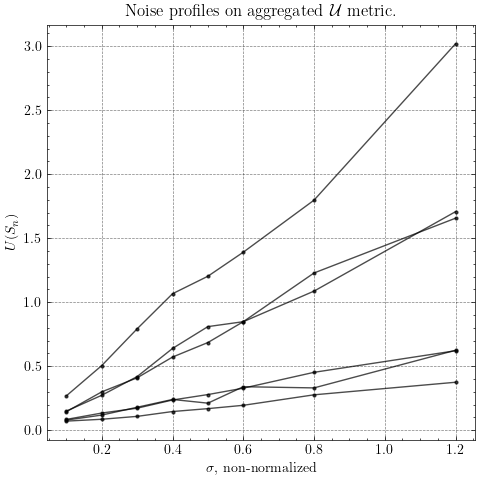
\includegraphics[width=0.5\textwidth]{img/uncertainty_U_linearized.png}
%    \caption{Noise uncertainty creation, aggregated through the metric $\mathcal{U}(\mathcal{S}'_{n})$ of the diffused %dataset. Here, we can see that for $y$-only corrupted noise, the uncertainty increased on bounding for $2\sigma^{2}%$, of which diverges several noise profile from one another. An interesting outlier is in the supressing effect of %mean-scale additive noise, which is not as expected.}
%    \label{fig:uncertainty_condition_1}
%\end{figure}

\begin{figure*}
    \centering
    \begin{tabular}{cc}
    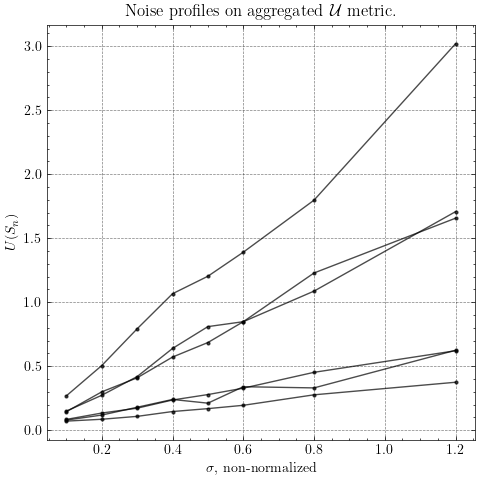
\includegraphics[height=0.25\textheight]{img/uncertainty_U_linearized.png} &
    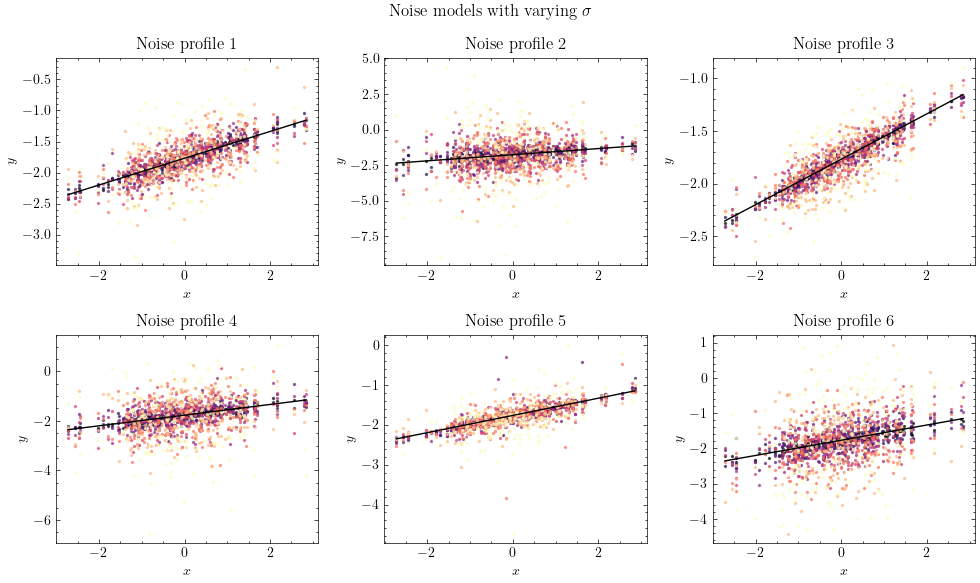
\includegraphics[height=0.3\textheight]{img/ETP1.png} \\
    {\bf (a)} & {\bf (b)}
    \end{tabular}
    \caption{Noise uncertainty creation, aggregated through the metric $\mathcal{U}(\mathcal{S}'_{n})$ of the diffused dataset. Here, we can see that for $y$-only corrupted noise, the uncertainty increased on bounding for $2\sigma^{2}$, of which diverges several noise profiles from one another. An interesting outlier is in the suppressing effect of mean-scale additive noise, which is not as expected.}
    \label{fig:dataset}
\end{figure*}

In general, noise are typically of consideration from two testing apparatus perspectives. First, is the \textit{empirical laboratory consideration}, or supposedly full-control in designer's corruption mechanism and intervention on the observations given; the second one being \textit{blind noise consideration}, in which noise is treated to be irreducible, of no origin and in which contributes only distortion on the dataset itself, without structural reason. As for such, how the dataset is interpreted depends on what version of the two extreme one take on the realization of the dataset itself, such is to say a way to analyze the dataset, within various statistical methods, or structural one. 
\begin{figure}[htb]
    \centering
    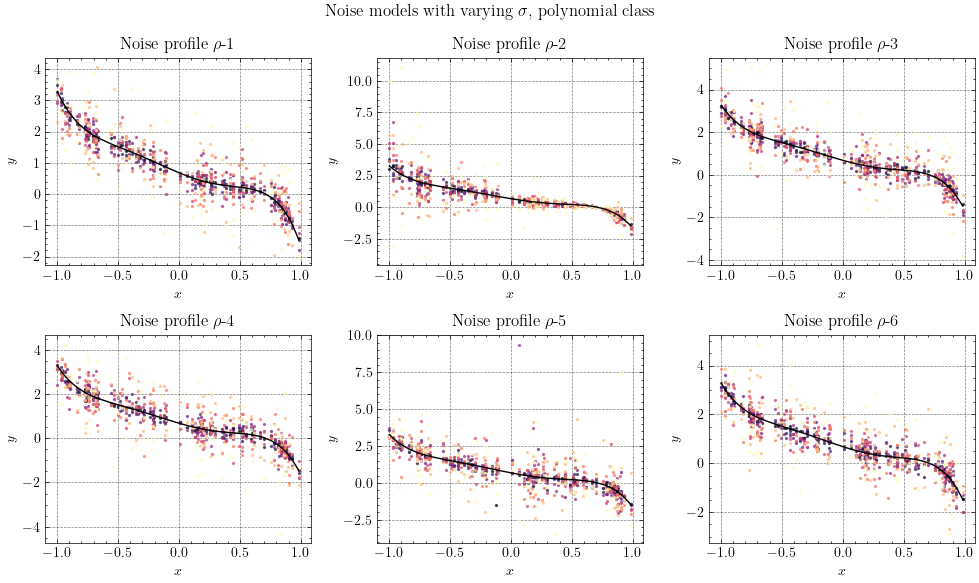
\includegraphics[width=0.8\textwidth]{img/poly_dataset.png}
    \caption{The different variations of the noise profile that can be often seen when sampling from a polynomial model, particularly constrained, 5th degree $p_{5}$ univariate polynomial on $[-1,1]$ domain inverse range. By order, (1) represents mean-scale additive noise, (2) considers heteroskedastic multiplicative noise, (3) considers variance-scaled additive noise, (4) considers absolute additive noise (where scale independent of $y$), (5) considers heavy-tailed noise (Student-$t$ modelling), and (6) is the standard canonical Gaussian noise (basically the default). We can see that each distributive pattern produces various different, often irreducible to Gaussian noise configurations.}
    \label{fig:generative_dataset_condition_poly}
\end{figure}

Aside from the main statistical approach, of which can be considered in many different ways, most often probabilistic-random variable approach to data extrapolation, the space encoding of the dataset itself is often very much interesting on itself, especially for a learner expression that would approximate such concept. Since we already used an illustration of the rather more complex notion of computational systems, we would like to use that in-effect of one of the notion of sample space analysis, i.e. the uncertainty metric $\mathcal{U}$. 

Polynomial regression is then one such analytical solution to function approximation task, using Weierstrass theorem as its basis. From such, we can also observe that polynomial regression, and hence polynomial interpolation, are correlated and can be reduced to each other. Polynomial regression can be reduced to interpolation via stating the criteria such that, denoting it as $\ell$, then $\ell(f,p)=0$, and interpolation can be reduced to regression via the condition that $p(x_{i})-y_{i}\leq \epsilon$ for arbitrary $\epsilon>0$. Hence, the regression formulae lie between the two extreme: the Weierstrass setting and the interpolation setting. 

We then have to identify such extreme and what kind of extreme they represent. Fortunately, we know this as the problem of \textbf{transparency}, in the setting of approximation, which certainly correlates to the learning theory. According to such, the Stone-Weierstrass represents the total transparency case, where the function $f$ is known to the approximator with polynomial class. Interpolation represents total black box, where the goal is only to interpolate the sample point by itself. In between such interpretation, there exists a fundamental assumption, hence the structural assumption. 

\begin{assumption}[Transparency]
    For any bivariate pair $(x,y)$, we assume each pair depends on and originate from a based concept $y=f(x)$. 
\end{assumption}

Two kinds of knowledge is then available, which correlates to the degree of freedom the observation space can have. First is the knowledge of $f$. This knowledge of $f$ is encoded directly by the number of sample point and their distribution in certain case. Accordingly, the worst case is as followed. 

\begin{conjecture}
    If $\forall x$ there exists $y$ corresponding to such, and $(x,y)\in \mathcal{S}$, then we say we have total transparency to the concept $f$. If there exists only finite $x$ that we can have $y$ corresponding to, then we say we have limited transparency to the concept $f$. If we assume no knowledge of $f$, then we say the setting is called the \textbf{black-box setting}. 
\end{conjecture}
Secondly, is the action on the dataset itself and what kind of concept is used to model the given structural observation. One of the main assumption that is usually observed is that, we presuppose a specific structures that after a finite amount of iteration, can return us back the desired results. 

\begin{assumption}[Fallacy]
    We assume there exists every specific bivariate pair $(x_{i},y_{i})\in f[\mathcal{S}_{n}]$, such that $f(x_{i})=y_{i}$. 
\end{assumption}

However, usually, this is not the case, as we have \textbf{noise} in addition from the dataset. The origin of the noise cannot be tracked. However, we can interpret what happens when such noise is introduced to the dataset. The noise transitions the transparency of the learned setting, on the field $\mathbb{R}$, by utilizing the dense property of the real space. Assuming we operate on $\mathbb{Z}$. Then, each discrete noise will introduce abnormality point such that no function on $\mathbb{Z}$ will be able to match, up to certain distance on $\mathbb{Z}$. This is because on such space, there exists no point $x_1, x_{2}$, for example, that lies between $d(x_{1},x_{2})=1$. If the noise is randomized on $\pm 1$, then there will exists no function that can approximate such disparity better than a random fluctuating function. However, on $\mathbb{R}$, the real number is inherently dense, such that there will always be certain point $x_{3}$ such that $x_{3}\in [x_{1},x_{2}]$, by the density of real number. By the distance metric on $\mathbb{R}$, we define $d(X,Y)=|X-Y|$ for distance between two data points. Noise intrinsically increases such distance, such that $d'(X,Y)> d(X,Y)$. Hence, the space in which density can appear increase, thus there then exists more fluctuation, and thus more uncertainty between such two points. This notion can be increased from local uncertainty to global uncertainty, hence the \textit{noisy dataset}. 

We then can measure or aggregate some properties of the dataset itself, including the \textbf{uncertainty} of the dataset. We define the simple uncertainty of the dataset as followed. 

\begin{definition}[Dataset uncertainty]
    Given a closed interval $[a,b]$, for the sample set $\mathcal{S}_{n}=(X,Y)\in [a,b]$, the uncertainty $\mathcal{U}(\mathcal{S}_{n})$ is defined as 
    \begin{equation}
        \mathcal{U}(\mathcal{S}_{n}) = \left[ \underset{x_{i}\in X}{\mathbb{E}}\Big( x_{i+1} - x_{i} \Big)^{2} + \underset{y_{i}\in Y}{\mathbb{E}} \Big( y_{i+1}- y_{i} \Big)^{2} \right]^{1/2}
    \end{equation}
    We assume $X,Y$ are totally ordered sets. 
\end{definition}

Hence, the assumption of fallacy assumes $\mathcal{U}(\mathcal{S}_{n})=0$, though in reality it is often $\mathcal{U}(\mathcal{S}_{n})>0$. We would like to clarify, that such definition is currently reserved for only polynomial-like functional class; though, this can be extended pretty easily for any $\mathbb{R}^{n}\to\mathbb{R}^{m}$ functional concepts. Furthermore, it is \textit{operational}, in the sense that it measures the numerical encoding inherent uncertainty, of which is also the space used of algorithms traversing in stochasticity. It affects cross-validation, gradient-based algorithm path finding, and roughness of the learning processes. Certain concerns must also be addressed, such as the definition, which assumes \textit{sequential processing} and pair-wise measurement (which can also be extended to tri-fold measurement and so on). Indeed, modern deep learning use parallel batch processing, mini-batch sampling, or distributed learning across devices for optimization. Nevertheless, such includes sequential-based learning optimization, and so on, where mini-batch still inherently includes batch ordering; algorithms like RNNs and so on also are sequential. The computational cost per dataset, if not, is $\mathcal{O}(n)$ after initial order, or with mundane immediate measurement on the way that the dataset was configured at start, since the system and stochastic algorithms sequentially go through them.

Certain others aspects can be expected to be clarified. While indeed, this is order-dependent measure, and one might expect to go against it and say it is not real dataset property, but the key point is that dataset are measurements, captured and recorded into the encoded space that is used upon the learning regime (supervised or semi-supervised or so on), or the learning algorithms. In a classical algorithmic world, such must be done in discrete steps, and hence ordering strongly matters as well as the processing pipeline relevant to it. There exists natural ordering of data within noise $\epsilon$, because if now, the projection on embedded space $\mathbb{R}^{n}\times \mathbb{R}^{m}$ of any given concept functional $c$ holds no value, as the function itself, plus the distribution, with respect to the encoding space where the function mapping is defined already contains structural information encoded within 'value range' as the most basic form. A weaker posture we can adopt is that it is an operational uncertainty measure, given presentation order to a finite discrete processing machine, and is indeed \textit{pre-training} diagnostic. There is also the issue in which $X$ and $Y$ might not be measurable or comparable. Indeed, since the range of value can jump intermittently between different concept class and form, but even then, it will only highlight the disparity between the contributing terms. For example, if we have three pairs, $(130,1)$, $(150,1)$ and $(225,0)$ as the data, then the volatility is not that bad, and stable on $Y$, but \textit{very high on $X$}, as there are missing information in large gap. From the machine-algorithmic, this matters. if we take the $130,225$ points as a case of shuffling, then the machine experiences a 95-to-1 volatility ratio. Nevertheless, one can attempt a normalized metric, i.e. 
\begin{equation}
    \mathcal{U}_{\mathrm{norm}}(\mathcal{S}_{n}) = \sqrt{\mathbb{E}[(\Delta x_{i})/r(X)]^{2}+\mathbb{E}[(\Delta y_{i})/r(Y)]^{2}}
\end{equation}
for relative jumpiness across different problems with normalized morphism. 
With this, we can quantify how the dataset is behaving on the scale of the bivariate form typically seen. Noise intrinsically increases this distance, usually by the $y$-axis. This dataset uncertainty increases with multivariate dataset, for example, $(\mathbf{x},y)$ of $\mathbb{R}^{n}\to\mathbb{R}$. We call the new metric as the \textit{empirical uncertainty metric}. The basis of such argument on the concept of a tradeoff comes from \cite{nakkiran2019datahurtlinearregression}, in which linear regression is affected, at least in such setting and consideration, such that dataset will both hurt and benefit the learning process. 

Overall, however, this allows us to state of the following theorem: 

%\begin{theorem}[Separation encoding]
%    We fix the encoding space on $\mathbb{D}=\mathbb{R}^{q}\times\mathbb{R}^{p}$ for a $(q,p)$ conjunction space. For $\mathcal{S}_{n}\in\mathbb{D}$ of $n$ samples $(x_{i},y_{i})$, we assume such set is output from an oracle $EX(\theta)$. Then, for a diffused set $\mathcal{S}_{n}'=\mathcal{S}_{n}+\eta$, for $\eta=\mathcal{D}\approx \mathcal{N}(0,\lambda\sigma^{2})$, then
%    \begin{equation}
%        \underset{\eta \in \{\mathcal{N}\}}{\mathbb{E}} [\mathcal{U}(\mathcal{S}_{n}')] \geq \mathcal{U}(S)
%    \end{equation}
%    for $\lambda \sigma^{2}$ the $x$-aware deviation. Fix $\lambda=1$ for consistent enclosure $0$-based error, or $\mathcal{N}(\cdot,\sigma^{2})$ for consistent data deviation. 
%\end{theorem}

\begin{theorem}[Separation Encoding under Diffusion]
    Fix the encoding space $\mathbb{D} = \mathbb{R}^{q} \times \mathbb{R}^{p}$ 
    for a $(q,p)$ conjunction space. Let $\mathcal{S}_{n} = 
    \{(x_i, y_i)\}_{i=1}^{n} \in \mathbb{D}$ be a dataset of $n$ ordered 
    samples drawn from an oracle $EX(\theta)$. Let $\{\mathcal{N}\}$ denote 
    the set of noise configurations $\eta = \{\eta_i\}_{i=1}^{n}$ where each 
    $\eta_i \sim \mathcal{D}$ with $\mathbb{E}[\eta_i] = 0$ and 
    $\mathbb{E}[\eta_i^2] = \sigma^2 < \infty$, independent across 
    components. Define the diffused dataset 
    $\mathcal{S}_{n}' = \{(x_i + \eta_i^{(x)}, y_i + \eta_i^{(y)})\}_{i=1}^{n}$. 
    Then
    \begin{equation}
        \underset{\eta \in \{\mathcal{N}\}}{\mathbb{E}}
        \left[\mathcal{U}(\mathcal{S}_{n}')^{2}\right] 
        = \mathcal{U}(\mathcal{S}_{n})^{2} + 4\sigma^{2}
    \end{equation}
    In particular, for any $\sigma^2 > 0$ and any zero-mean 
    finite-variance $\mathcal{D}$,
    \begin{equation}
        \underset{\eta \in \{\mathcal{N}\}}{\mathbb{E}}
        \left[\mathcal{U}(\mathcal{S}_{n}')^{2}\right] 
        > \mathcal{U}(\mathcal{S}_{n})^{2}
    \end{equation}
\end{theorem}

\begin{proof}[Proof 1. Simple proof]
    Using normed metric, $\mathcal{U}_{\mathrm{norm}}$. For noised data, that is, \begin{equation}
        \mathcal{S}_{n}' = \{(x_{i}+\eta^{(x)}_{i}, y_{i}+\eta^{(y)}_{i})\}^{n}_{i=1}
    \end{equation}
    where the noise vector on encoding space is orthogonal, such that \begin{equation}
        \eta_{i}=(\eta_{i}^{(x)},\eta_{i}^{(y)})\sim\mathcal{D}\approx \mathcal{N}\left(a,\lambda\mathrm{Cov}(\eta)\right)
    \end{equation}
    where we can fix $\mathcal{D}=\mathcal{N}(a,\lambda\sigma^{2})$ for $a=0$ as normalized around the zero value. If we assume independent noise, then we have the covariance as 
    \begin{equation}
        \lambda \mathrm{Cov}(\eta)= \lambda\begin{pmatrix}
            \sigma_x^2 I_q & 0 \\
            0 & \sigma_y^2 I_p
        \end{pmatrix}
    \end{equation}
    We can simplify slightly, as to have the case in consideration that $\sigma^{2}_{x}=\sigma^{2}_{y}=\sigma^{2}$, then the notation would effectively be such that $\lambda\sigma^{2}I_{d+p}$ is enough. The uncertainty metric then should be expressed as 
    \begin{equation}
        \begin{split}
            &\mathbb{E}[\mathcal{U}(\mathcal{S}_{n}')^{2} ] \\
            &= \mathbb{E}\left[\underset{x_{i}\in X}{\mathbb{E}}\Big( x_{i+1} - x_{i} \Big)^{2} + \underset{y_{i}\in Y}{\mathbb{E}} \Big( y_{i+1}- y_{i} \Big)^{2}\right]\\
            & = \mathbb{E}_{i}\left[ (x_{i+1}'-x_{i}')^{2} \right] + \mathbb{E}_{i}\left[ (y_{i+1}'-y_{i}')^{2} \right]
        \end{split}
    \end{equation}
    for $\mathbb{E}_{i}$ here denotes the expectation over the uniform index $i$ of each component of the sample space. Now, we substitute the following into the empirical average pair:
    \begin{equation}
        x_{i+1}'- x_{i}' = (x_{i+1}- x_{i}) + (\eta_{i+1}^{(x)}- \nu_{i}^{(x)}), \quad y_{i+1}'- y_{i}' = (y_{i+1}- y_{i}) + (\eta_{i+1}^{(y)}- \nu_{i}^{(y)})
    \end{equation}
    First, for $x_{i},x_{i+1}$ set, taking expectation over noise $\eta$ gives
    \begin{equation}
        \begin{split}
            \mathbb{E}_{\eta} \left[ (x_{i+1}'-x_{i}')^{2} \right] 
            &= \mathbb{E}_{\eta} \left[ (x_{i+1}-x_{i})^{2} + 2(x_{i+1}-x_{i})(\eta_{i+1}^{(x)}-\eta_{i}^{(x)})+ (\eta_{i+1}^{(x)}-\eta_{i}^{(x)})^{2} \right] \\
            & = \mathbb{E}_{\eta} \left[ (x_{i+1}-x_{i})^{2} + (\eta_{i+1}^{(x)}-\eta_{i}^{(x)})^{2} \right], \qquad \mathbb{E}_{\eta}\left[2(x_{i+1}-x_{i})(\eta_{i+1}^{(x)}-\eta_{i}^{(x)})\right] = 0 \\
            & = \mathrm{Var}(\eta_{i+1}^{(x)}) + \mathrm{Var}(\eta_{i}^{(x)}) \\
            & = 2\sigma^{2}
        \end{split}
    \end{equation} 
    for $x_{i}$ fixed and $\mathbb{E}[\eta_{i}^{(x)}]=0$ that leads to the second zero equality, independent noise $\eta_{i+1}^{(x)},\eta_{i}^{(x)}$ with variance $\sigma^{2}$. Therefore, we have for each $i$ pairing, that
    \begin{equation}
        \mathbb{E}_{\eta} \left[ (x_{i+1}'-x_{i}')^{2} \right] = (x_{i+1}-x_{i})^{2} + 2\sigma^{2}
    \end{equation}
    Averaging over $i$ and apply the same argument to $y$-component, we gain identical form with doublecondition, such is, 
    \begin{equation}
        \mathbb{E}[\mathcal{U}(\mathcal{S}_{n}')^{2} ] = \mathbb{E}_{i}\left[ (x_{i+1}-x_{i})^{2} \right] + \mathbb{E}_{i}\left[ (y_{i+1}-y_{i})^{2} \right] + 4\sigma^{2} = \mathcal{U}(\mathcal{S}_{n})^{2} + 4\sigma^{2}
    \end{equation}
    Since $\sigma^{2}>0$, the expression gives $\mathcal{U}(\mathcal{S}_{n})^{2} + 4\sigma^{2}>\mathcal{U}(\mathcal{S}_{n})^{2}$ by Jensen inequality. The statement works under expectation in the squared sense directly, and for $\mathcal{U}$, we expect monotonicity on $\mathbb{R}_{\geq 0}$ for square terms reduces to the expression on non-squared condition.  
\end{proof}

Specifically, the unsquared version will give
\begin{equation}
    \mathbb{E}[\mathcal{U}(\mathcal{S}'_{n})] \leq \sqrt{\mathbb{E}[\mathcal{U}(\mathcal{S}_{n}')^{2}]} = \sqrt{\mathcal{U}(\mathcal{S}_{n})^{2}+ 4\sigma^{2}}
\end{equation}
which again, requires the argument going through the squared form by condition. The condition that invalidates the theorem under such form would be for any non-zero mean noise, for $\mathbb{E}[\eta_{i}]=\mu\neq 0$, which does not collapse the contributing terms. The middle $2\mu\cdot \mathbb{E}_{i}[\cdot]$ term then is a telescoping sum proportional by $(x_{n}-x_{1})/(n-1)$, which can be either positive or negative depending heavily on trend in $X$ space, so biased noise can actually \textbf{increase or decrease} uncertainty extrapolated depending on dataset structure. This is rather interesting, because it highlights a particular region where systemic bias (or so we called of such), interacts with dataset ordering in a non-trivial way, which is far harder to concentrate. In fact, the real form under arbitrary notion can be written as 
\begin{equation}
    \mathbb{E}_{\eta}[\mathcal{U}(\mathcal{S}_{n}')^{2}] = \mathcal{U}(\mathcal{S}_{n})^{2} + 2(1-\rho)(\sigma^{2}_{x}+\sigma_{y}^{2}) + \mathrm{Bias}
\end{equation}
of the bias term arbitrary, and covariance $\rho\sigma^{2}$ for correlation of both $\eta_{i},\eta_{i+1}$, which is rather interesting, and targets the case of sensor drift in observational spaces. Finally, the constraining partition is that if we have infinite variance on $\mathcal{D}$, then the finiteness of $\mathcal{U}(\mathcal{S}_{n}')$ is not finite and the comparison is undefined. As such, while interesting, and indeed extensible to a wider variety of control space for dataset, we note the inherent understanding and restriction of such uncertainty measure. 

Such type of experimental pre-pipeline investigation can also be very informative on the structure of the dataset in whole, particularly within the tension of \textbf{dataset identifiability}\index{dataset identifiability} projection. Specifically, it is where we are to hinge upon the two perspective on absolute noise independency from structures, or structural noise, of which would be rather difficult to approach form. This can be raised of the problem as followed. In a specific dataset, between the \textit{actual concept} and the observable spaces, lies the empirical and generalization setting. While it is not often mentioned in literatures, the switch to direct observable evaluation of statistical learning, induces certain limitations that would determine how any specific dynamical system operate under its domain, and of which the data points itself, i.e. here we call it as observational points of the observation space, be inferred of one another, or our dataset being a snapshot of a limited frame in which the dynamics are frozen in capture. 

Let us assume the following preliminary in discussion. We have two polars, on the mechanistic absolute, or \textit{white box} knowledge, with full expressions on the underlying mechanics of a certain system concept. Explicitly, this can be written as $y=F(x;\theta)$ under standard morphism, for any kind of description $\theta$. Extension of such notion can also include what we call as the mechanism, or $F(x;\theta,\Gamma)$ of which complies both the parameters, and the formulations. The other polar is the \textit{probabilistic domain}, of which then, we have the inference $\sim$ operator instead. Thus, we denote $y\sim \mathbb{P}(Y\mid X)$ in typical notation, in which the dependency is now $Y$ on the basis of $X$. One can also do the reverse, as to generate the inverse conditions, but this is more probably general, if one switch to joint distribution $(X,Y)$ under statistical schemes. Abstractly speaking, the dual structure contains what we call temporary, as the \textbf{system action} $A_{S}$. The notation then becomes 
\begin{equation}
    yA_{S}x \to f(x;\theta,\Gamma), \quad yA_{S}\to \mathcal{S}[\mathbb{P}(X,Y)]
\end{equation}
For $\mathcal{S}$ here temporarily denotes the \textit{sampling operations}, of observing randomly on the basis of said probability without any knowledge but the presumed parameters. If such process is with control parameter, from the optimization perspective, we have the notation as different to be $\mathcal{S}[\mathbb{P}(X,Y);\theta_{P},\Gamma_{P}]$, where now $\Gamma_{P}$ is the probabilistic process, i.e. distributions or other random structure, for example as stochastic processes as a finite-dimensional distributions plus regularity structure, for random variables $\theta_{P}$. In general, we call it the \textbf{black-box} domain. 

If we are to recover $\theta$ from $\theta_{P}$, or at least on the similarity metric, typically or ML encoded by $\ell(\theta,\theta_{P})$, where $\ell(\theta,\theta_{P})\approx 0$, then we say that the system experiences a \textit{white transition}. Note that we do not take into account of $\Gamma$ and $\Gamma_{P}$, since they are inherently different in this white transition, but mechanistically recoverable; thus, \textit{total white transition} means $\Gamma \approx \Gamma_{P}$ of the mechanistic patterns. If the reverse happens, where mechanistic system turn to probabilistic $(X,Y)$ distribution on $\theta_{P}$ and structure $\Gamma\to\Gamma_{P}$. 

Probability inherently, similar to mechanistic $\Gamma$, enforces causal or rather transformational relation (simply the dual $x\to y$ is transformational within $f$). There, the probability can be interpreted, for either $\Gamma$ explicitly states that they are conditional, for $X$ to be deterministic and explicitly stated, or joint distribution and so on. However, the interference in such recovering mode comes from observational space inconsistency. This is usually expressed of \textit{noise}, where if we admit $(x,y)$ of the mechanistic system, then for $x+\epsilon_{x}$ and $y+\epsilon_{y}$ we have instead a \textit{noisy mechanistic system}. We would note that this is a larger class than pure mechanistic system, basically $x\to [\epsilon, f(x;\theta,\Gamma)]$ instead. Thus, for intrinsic noise of measurements or statistical information, probabilistic transition in recovery of mechanistic systems admits the recovery of the noisy system instead. Depends on the severity of $\epsilon$, such system can be irrecoverable. If such approximation is impossible within certain margin, then probabilistic approximation remains in probable the only manageable system of approximation, rather than a quasi mechanistic recovery mode (we will prove this in a later theorem). If we to accept such view, then it means that in certain failure modes, you \textit{cannot move a mechanistic (deterministic) system into probabilistic then back}, given enough disturbance and noise. This quantifies to the \textit{information loss} system-wide, where we can create a prototypical functional, denoted $\mathcal{R}:F\to P$, where
\begin{equation}
    \mathcal{R}[F](A) = \int_{\Theta} \bf{1}_{\{F(x;\theta,\Gamma)\in A\}}\mu (d\theta)
\end{equation}
for such transition, of the probabilistic measure space $(\Omega, \mathcal{F},\mathbb{P})$, for $\mu\in \mathcal{F}$ and $A\in(\mathcal{X},\mathcal{Y})$ of the observational space. The implication here is that, under no information (information-agnostic), every noisy concept must meet certain limit on the basis and resultant structure itself. There exists, presently, no sufficient guarantee to return $P$ to $F$, except the same operation in reversal, is forced on ideal setting, for infinite-range coverage, and approximately dense observational space. The limit is, inherently, enforced by arbitrary $\epsilon$. It is to note that we do not claim that mechanistic systems are ontologically privileged; we claim that the mapping from mechanisms to observations is not generally invertible under disturbance. Thus, effectively, what we have done is simply the motivation for said approach, and the importance of considering the entire dataset space rather than just aggregated on value-specific distribution under measurements. 
\section{Linear function class $h(u)$ - \cite{lafon_understanding_2024}}

Linear-linear scenario learning is one particularly well-studied case of representing double descent or not, usually through simplicity in analysis (of the similar ease of proof compared to binary classification). Models in this setting can be said to share the same \textit{parameter space} with no additional structure or scaling mask (like in monomial basis). The model that is representative of this preliminary observation is from \cite{lafon_understanding_2024}, specifically, linear regression (function approximation) with Gaussian noise, and of univariate case. Consider the family class $(\mathcal{H}_p)_{p\in\llbracket1,d\rrbracket}$ of linear functions $h:\R^d\mapsto \R$ where exactly $p$ components are non-zero ($1\leq p\leq d$), we have the following model.

\begin{definition}[\cite{lafon_understanding_2024}]
For $p \in \llbracket1,d\rrbracket$, $\mathcal{H}_p$ is the set of functions $h:\R^d\mapsto \R$ of the form:
$$
h(u)=u^Tw,\quad \text{for }u \in \R^d
$$
With $w \in \R^d$ having exactly $p$ non-zero elements. The complexity here itself can be interpreted as the effective random initialization, trimming down data of hidden details instead - this is indicated by the amount of information it observes given $d$ dimension, and $p$-hypothesis dimension. \footnote{According to the \textit{manifold hypothesis}, there are chances where the actual concept can be interpreted and mimicked by seeing that it lies on a lower-dimension manifold inside its actual expressive dimensional space. }
\end{definition}
Using such model, they consider the setting of minimizing the customized mean square loss, 
\begin{equation}
\label{eq:linear_gaussian_erm}
\min_{w\in \R^d} \frac{1}{2}\norm{\bm{X} w - \bm{Y}}^2 \to \min_{w\in \R^p} \frac{1}{2}\norm{\bm{\Xp} w - y}^2
\end{equation}
of the sub-problem on $p$ cardinality, where again $p$ is the dimensionality or independent degree of freedom. This results in the following theorem that 'mimic' double descent on this linear regression model.

\begin{theorem}[Double descent on linear regression - \cite{lafon_understanding_2024}]
\label{thm:double_descent_lr}
Let $(x, \epsilon)\in \R^d\times\R$ independent random variables with $x \sim \mathcal{N}(0,I)$  and $\epsilon \sim \mathcal{N}(0,\sigma^2)$, and $w \in \R^d$. we assume that the response variable $y$ is defined as $y=x^Tw +\sigma \epsilon$. Let $(p,q) \in \llbracket 1, d\rrbracket^2$ such that $p+q=d$, $\bm{\Xp}$ the randomly selected $p$ columns sub-matrix of X. Defining $\hat w:=\phi_p(\p{\hat w},\q{\hat w})$ with $\p{\hat w}=\bm{\Xp}^+y$ and $\q{\hat w} = 0$.\\
The risk of the predictor associated to $\hat w$ is:
\begin{equation}
    \begin{split}
        &\E[(y-x^T\hat w)^2] \\
        & = \begin{cases}
(\norm{\wq}^2+\sigma^2)(1+\frac{p}{n-p-1}) & p\leq  n-2\\
+\infty &n-1 \leq p\leq  n+1\\
\begin{split}
    &\norm{\wp}^2(1-\frac{n}{p}) \\
    &\quad +  (\norm{\wq}^2+\sigma^2)(1+\frac{n}{p-n-1})
\end{split} &p\geq n+2\end{cases}
    \end{split} 
\end{equation}
The point $p=n$ is representative of the interpolation threshold from underparameterization to overparameterization. 
\end{theorem}

We present two parts - first are those fundamentals predicted by the theorem, and second are verifications of the theorem with our own version of testing. The first experimental setting is then conducted with fixed $d$, varying $p$ for each varying $n$ samples. Since this is a least square result, preliminary run is conducted using one-shot error-risk measure on least square closed-form approximation. Note that $p\leq d$, hence we are regarding the domain of the term underparameterized and equal parameterization setting. The result is presented in Figure~\ref{fig:theorem_double_descent_fig}

\begin{figure}[htb]
    \centering
    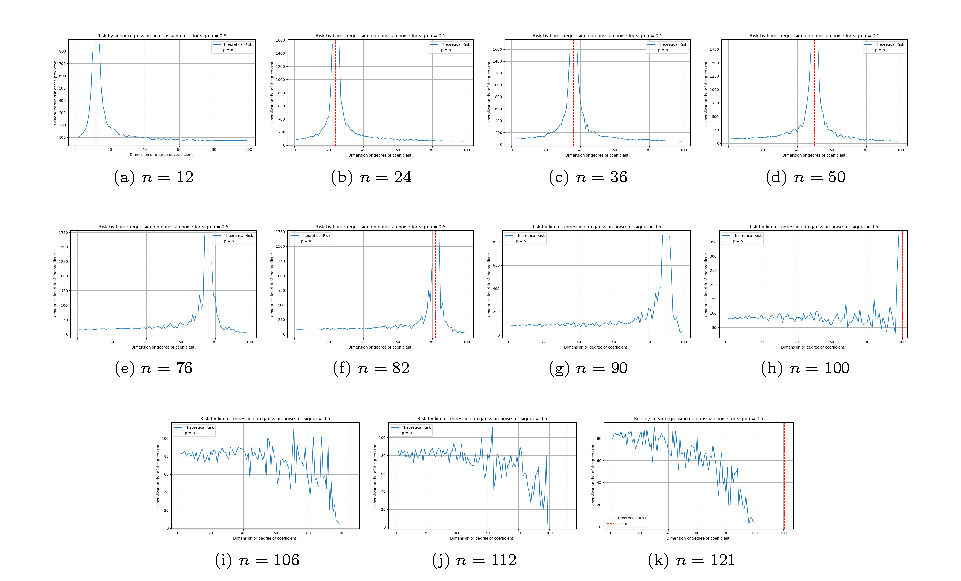
\includegraphics[width=0.8\textwidth]{pdf/theorem_1.pdf}
    \caption{Theorem~\ref{thm:double_descent_lr} behaviours on randomized setting. For this model, we have $d=100$, $\sigma = 0.5$, and variational $n$. Full test cases are for $p=[1,100]$, $n=\{12,24,36,50,76,82,90,100,106,112,121\}$ accordingly. The test function of the concept itself is the same linear model, but with different input only.}
    \label{fig:theorem_double_descent_fig}
\end{figure}

As we see from this particular experimental result, the theorem predicted a loose, left-peak absent, double descent curve estimation for a variety of test case with more and more samples in increment. There exist some fundamental conclusion that we have about the shift of the interpolation threshold upon to $p=n$, which is reflected in the piecewise prediction. However, this pattern breaks down for $n$ higher than specific constant, for this case, starting from $n\approx 100$ to beyond. From here, at least from testing scenario, the test indicates that predictions suggest a breakdown of the double descent estimation. Beyond this, a simple semi-chaotic convergences is observed, from $n=106,112, 121$. 

Interestingly, verifying this notion of easy enough to simplify it into what the statement holds under particular notion. Namely, as we find out, the above double-descent replicating formula can actually be realized by the parameter-wised error, comparing the parameter between the least-square solution and the actual concept. The formula for this is expressed by the exposed MSE on parameter function, for $\beta_{p,k}$ the coefficient value estimated for the $k$-th selected feature when the model is restricted for randomization of $p$ features, 
\begin{equation}
\mathrm{MSE}_{\mathrm{param}}=\left\lvert \hat w - w \right\rvert _{2}^{2}=
\sum_{j=1}^{d}
\left(
  \hat w_{j} - w_{j}
\right)^{2}
\end{equation}
where $\hat w_{j}$ is chosen such that it is equal $0$ for $j \notin S$, otherwise $\beta_{p,k}$ for \(S=\{i_1,\dots,i_p\}\) is the set of selected feature indices. Nevertheless, it is then found dubious why this is true, as for the original statement of \cite{lafon_understanding_2024} indicates correlation to the prediction error of the result, $x^{\top}\hat{w}$ instead. The result of evaluating $\mathrm{MSE}_{\mathrm{param}}$ is presented in Figure~\ref{fig:theorem_double_descent_fig2}.

\begin{figure}[htb]
    \centering
    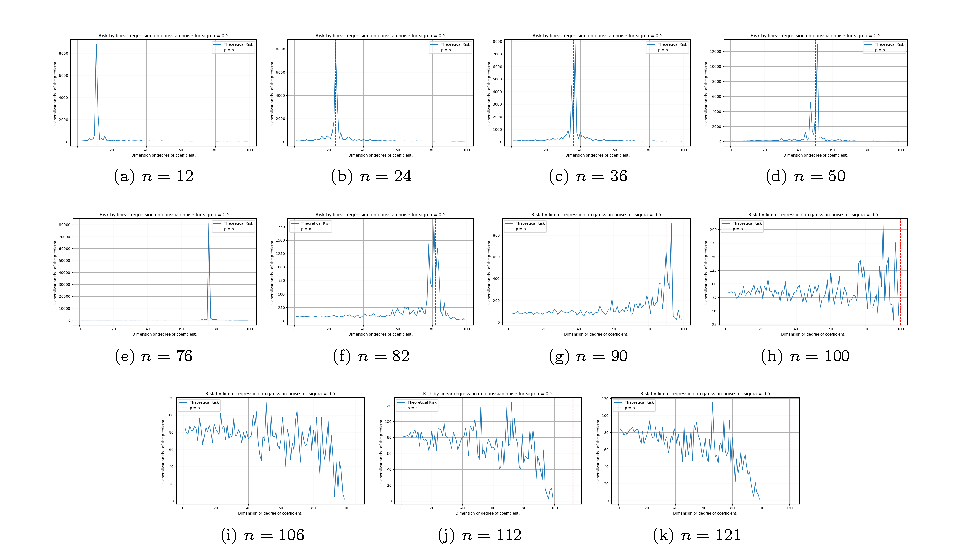
\includegraphics[width=0.8\textwidth]{pdf/theorem_2.pdf}
    \caption{Contrary to Theorem~\ref{thm:double_descent_lr}, this is the behaviours on randomized setting for standard parameter-wised mean square error measure (MSE-on-parameter). For this model, we have $d=100$, $\sigma = 0.5$, and variational $n$. Full test cases are for $p=[1,100]$, $n=\{12,24,36,50,76,82,90,100,106,112,121\}$ accordingly. The test function of the concept itself is the same linear model, but with different input only.}
    \label{fig:theorem_double_descent_fig2}
\end{figure}

If, however, we turn our attention to the statement itself, of which refers to the prediction error $\mathrm{MSE}_{\mathrm{pred}}$, defined by the equation
\begin{equation}
\mathrm{MSE}_{\mathrm{pred}}
=
\frac{1}{n}
\left\lVert
  y - X_{p}\,\hat\beta
\right\rVert_{2}^{2}
=
\frac{1}{n}
\sum_{i=1}^{n}
\left(
  y^{(i)} - x_{p}^{(i)\,T}\,\hat\beta
\right)^{2}
\end{equation}
on $h$ and $c$ accordingly, a strong case of this happens to be not following the pattern indicted by the theorem. Rather than being the interpolation point of return, $p=n$ is now the convergence point of the prediction error instead. Test result is shown in Figure~\ref{fig:theorem_double_descent_fig3}.

\begin{figure}[htb]
    \centering
    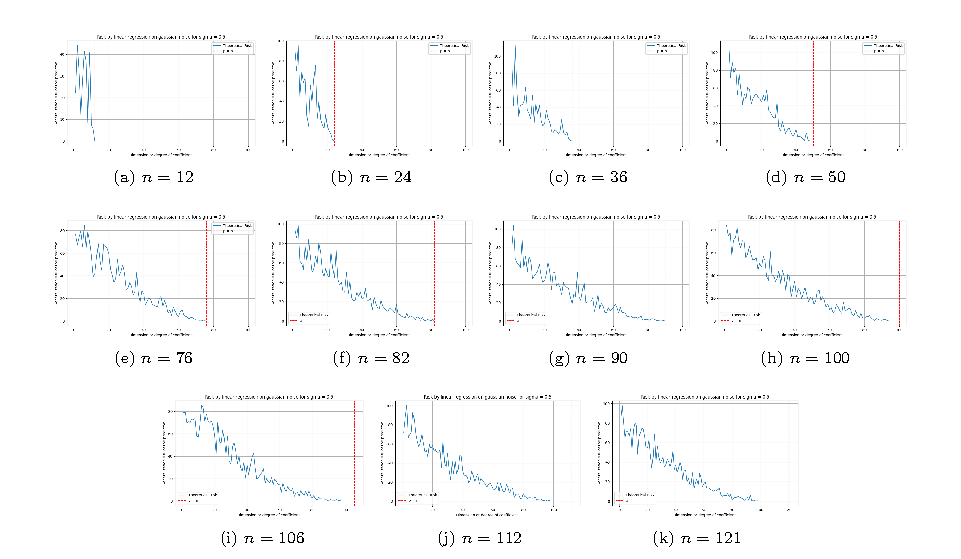
\includegraphics[width=0.8\textwidth]{pdf/theorem_3.pdf}
    \caption{Contrary to Theorem~\ref{thm:double_descent_lr} and both figure~\ref{fig:theorem_double_descent_fig2}, this is the behaviours on randomized setting for standard parameter-wised mean square error measure (MSE-on-prediction). Especially, we do not see double descent pattern in this setting, as it is. For this model, we have $d=100$, $\sigma = 0.5$, and variational $n$. Full test cases are for $p=[1,100]$, $n=\{12,24,36,50,76,82,90,100,106,112,121\}$ accordingly. The test function of the concept itself is the same linear model, but with different input only.}
    \label{fig:theorem_double_descent_fig3}
\end{figure}
\begin{figure}[htb]
  \centering
  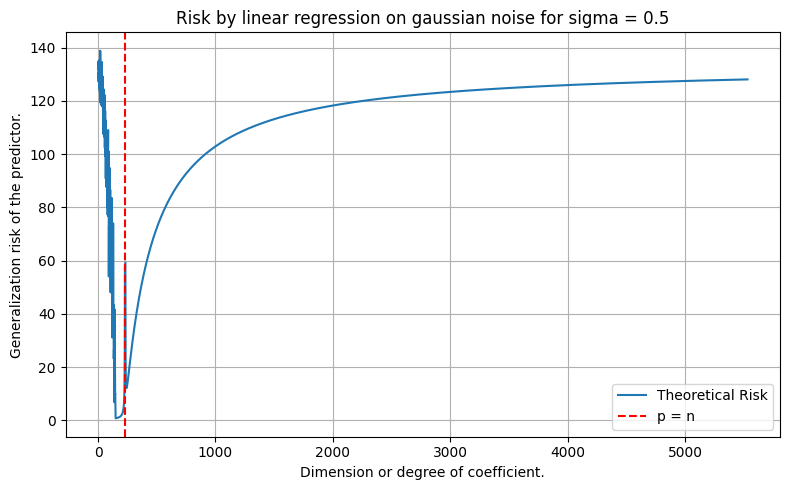
\includegraphics[width=0.6\textwidth]{media/dimensional_descent.png}
  \caption{Similar experiment according to setting and result of Theorem~\ref{eq:linear_gaussian_erm}, where $p$ is in the range $[1,5523]$. Here, we can see small double descent modelled exactly at the interpolation threshold, while the later region exhibit similar phenomenon as bias-variance tradeoff.}
  \label{fig:contrarian}
\end{figure}
Thence, the theorem gives us two things - the interpolation point, in this setting, refers to the parameter error for their double descent behaviour. However, on the prediction results' error measure, the interpolation point correlates to the point where the defined generalization risk in such case equals zero. These patterns hold up to certain point. However, the test case is only up to $d=p$. An unexplored test case for $p>d$ indicate the surprising fact according still, to the theorem: the generalization risk takes double descent as a region with disturbance in the middle, but bias-variance appears afterward. This is illustrated in Figure~\ref{fig:contrarian}, where the same theorem is applied but in the domain which is usually called as \textit{overparameterized region}. 

Such can then be seen as a prediction that double descent in certain case, can be extrapolated to be the transition between the two curvature of bias variance, or the abnormal point on the error curve measure. Such must then be verified, both in the experiment's correctness, and so on that lead to such result. Nevertheless, if true, it would mean that double descent indeed has another implication of itself. 

\subsection{Extension}

The current theory prompted for a more general treatment of the linear function class, as in-line with exploring reasonable existing alternatives in interpretation (\cite{nakkiran2019datahurtlinearregression}). We have much to desire of, for example, extension of prediction for stochastic or iterative algorithms, consideration on statistical formations, uncertainty metrics. Or furthermore, different kind of linear models, including multilinear models and so on, with variational setting meaningful to the problem space. 

Let us state some hypotheses about the previous experimental cases. First, is the lack of the begin-tail of the prediction on double descent of linear random cutoff features model. This can be explained informally as to be resulted from the uniformity of the operating space. Specifically, all parameters of the $\mathbb{R}^{n}$ parameter space, with respect to the dual space on such $f:\mathbb{R}^{n}\to\mathbb{R}$ projection is defined, are of the same order of magnitude. That is, for $f_{i,k}(x),f_{j,k}(x)$ of arbitrary parameter indexing on the set $k$ of shared parameter choice, and $i\neq j$ being the distinct choice, then we say $f_{i,k}(x)=\mathcal{O}(f_{j,k}(x))$ of the growth of both function on value ranges. Approximately speaking, the choice of parameter does not dramatically growth to a point of no return, like in later examples of polynomial approximation model. Such special model of multi-variable linear projection of scalar output also reinforces the numeric growth of the numerical encoding expression on the hypothesis model. The behaviour of the MSE-on-parameter, the internal risk, is also explainable using the same notion, such is that for a black-box case approximation, such linear model does not allow for average parameter deviation per approximation to be oversaturated and skewed (for example, the degree of polynomial directly counteract this, by separating expressive complexity by growth degree). How such hypothesis can be evaluated, we will have to make it for the general extension experiment, which we will have to conduct. 

Let us define the more general class of linear model, denoted $\mathcal{H}_{L}$, in the following structure of the linear model. We also note that the previous linear class $\mathcal{H}_{p}$ only solves for the problem of underparameterized, hidden parameters $p'$. Let $k \in \mathbb{N}$ denote the number of input vectors, and let $\mathbf{u}_1, \mathbf{u}_2, \ldots, \mathbf{u}_k$ represent the input vectors where each $\mathbf{u}_i \in \mathbb{R}^{q}$ for $i \in \{1, 2, \ldots, k\}$. Here, $q \in \mathbb{N}$ denotes the dimensionality of each input vector, with the convention that $q = 1$ corresponds to scalar inputs (i.e., $u_i \in \mathbb{R}$).

For a given dimension parameter $d \in \mathbb{N}$, we define $\mathcal{H}_{L}$ as the set of all functions $h: (\mathbb{R}^{q})^k \to \mathbb{R}$ that can be expressed in the unified form:
\begin{equation}\label{eq:lin_extension}
        h(\mathbf{u}_1, \mathbf{u}_2, \ldots, \mathbf{u}_k) = \sum_{j=1}^{d} w_j \cdot \phi_j(\mathbf{u}_1, \mathbf{u}_2, \ldots, \mathbf{u}_k) + b
    \end{equation}
where $\mathbf{w} = [w_1, w_2, \ldots, w_d]^{\top} \in \mathbb{R}^{d}$ is the weight vector, $b \in \mathbb{R}$ is the bias term, $\phi_j: (\mathbb{R}^{q})^k \to \mathbb{R}$ is a feature map for $j \in \{1, 2, \ldots, d\}$ that transforms the input vectors into a scalar feature, we consider the following important special cases, distinguished by their choice of feature map $\phi_j$. If we do not have such feature mapping of which preserves relative linearity, then we said it is the basic linear class dynamic. 

\begin{definition}[Linear class, $q=1$]
    Consider class $h: (\mathbb{R}^{d+1})^{q}\to \mathbb{R}\in\mathcal{H}_{\mathsf{Lin}}$ of all functionals of the form as Equation~\ref{eq:lin_extension}. Then, when $q=1$ of scalar observables, i.e., $u_i \in \mathbb{R}$ for $i \in \{1, \ldots, k\}$, then the function is simply as:
    \begin{equation}
            h(u_1, u_2, \ldots, u_k) = \sum_{j=1}^{k} w_j \cdot u_j + b
    \end{equation}
    for $\phi_j(u_1, \ldots, u_k) = u_j$ for $j \in \{1, 2, \ldots, k\}$, i.e. deactive feature map. 
\end{definition}
Such class can be extended rigorously, through a varied change in dynamics, specifically, considering the general feature representation on $\phi$. 

\begin{definition}[General feature, kernel linear model]
    Consider class $\mathcal{H}_{\mathsf{Lin}}$. For maximum flexibility, allow arbitrary feature maps $\phi: (\mathbb{R}^{d+1})^{q}\times \mathbb{R}^{k}$ for $k=\{1,2,\dots\}$ as of hidden or feature mapping processor internally. The functional form is then expressed by 
    \begin{equation}
            h(\mathbf{u}_1, \mathbf{u}_2, \ldots, \mathbf{u}_k) = \sum_{j=1}^{d} w_j \cdot \phi_j(\mathbf{u}_1, \mathbf{u}_2, \ldots, \mathbf{u}_k) + b
        \end{equation}
        for $j\leq d$ as the iterative form. 
\end{definition}

Common choices for such kernel mapping includes:
\begin{itemize}[topsep=1pt,itemsep=1pt]
    \item \textbf{Polynomial features}: $\phi_j(\mathbf{u}) = u_{i_1} u_{i_2} \cdots u_{i_m}$ for various index combinations
    \item \textbf{Radial basis functions}: $\phi_j(\mathbf{u}_1, \mathbf{u}_2) = \exp(-\gamma \|\mathbf{u}_1 - \mathbf{u}_2\|^2)$
    \item \textbf{Fourier features}: $\phi_j(\mathbf{u}) = \sin(\boldsymbol{\omega}_j^{\top}\mathbf{u})$ or $\cos(\boldsymbol{\omega}_j^{\top}\mathbf{u})$
    \item \textbf{Neural network activations}: $\phi_j(\mathbf{u}) = \sigma(\mathbf{v}_j^{\top}\mathbf{u} + c_j)$ for activation $\sigma$, though we note that this is a very simplistic removal of structural basis class. Rather, it is performing shallow network in linear approximation on kernel system. The reason most of the time we do not use this is because of complexity in multi-kernel distortion. 
\end{itemize}
From such, it basically hints at the generality of, at least being a \textit{linear approximation} on various hypothesis spaces, while not actually being similar. Then, our setting of sparsity being synthetically induced introduces the basin of subclasses. For any $p \in \{1, 2, \ldots, d\}$, we can then simply define the sparse subclass $\mathcal{H}_{L,p} \subseteq \mathcal{H}_{L}$ as the set of all functions $h \in \mathcal{H}_{L}$ where the weight vector $\mathbf{w} \in \mathbb{R}^{d}$ has exactly $p$ non-zero entries. Formally, per \cite{lafon_understanding_2024},
\begin{equation}
        \mathcal{H}_{L,p} = \left\{ h \in \mathcal{H}_{L} : |\{j : w_j \neq 0\}| = p \right\}
\end{equation}
The subset $S \subseteq \{1, 2, \ldots, d\}$ of indices with $|S| = p$ corresponding to non-zero weights is assumed to be fixed throughout the learning process (i.e., the sparsity pattern is predetermined). This constraint yields:
\begin{equation}
    h(\mathbf{u}_1, \ldots, \mathbf{u}_k) = \sum_{j \in S} w_j \cdot \phi_j(\mathbf{u}_1, \ldots, \mathbf{u}_k) + b
\end{equation}
where only $p$ features contribute to the final prediction. This effectively masks the data randomly, simulating the general observation-based information corruptions, without inducing specific bias like \textit{dropout}, though potentially leads to strong perturbation in cases of meaningful information threshold for different function classes.

\subsubsection{Baseline investigations}

Preliminary model learning then will relies on theorem~\ref{thm:double_descent_lr} for its initial prediction, using least square approximation results. The testing is adversarial and consistent, of which we have $c\in \mathcal{H}_{L}$ and $h\in \mathcal{H}_{l,p}$ for $p=d$, which can then further be modified. Because of their equal expressive capacity, respect to independent consideration of the parameter space $\mathbf{X}$, we define the complexity, which will be used later on, simply as \begin{equation}
    \mathbb{C}(h) = \frac{1}{||\overline{\mathbf{x}}-\underline{\mathbf{x}}||}\left[1+p + q + \underset{i\in S}{\mathbb{E}} (w_{i}x_{i})+b\right],\quad S = \{p_{i}\} 
\end{equation}
Functional prediction on the classical theorem is presented below, for $n=\{1,\dots,241\}$ samples, and with $p\in[1,200]$. We set the target degree to the maximal 200, since the theorem is not defined on the overparameterized region. 

\begin{figure}[htb]
    \centering
    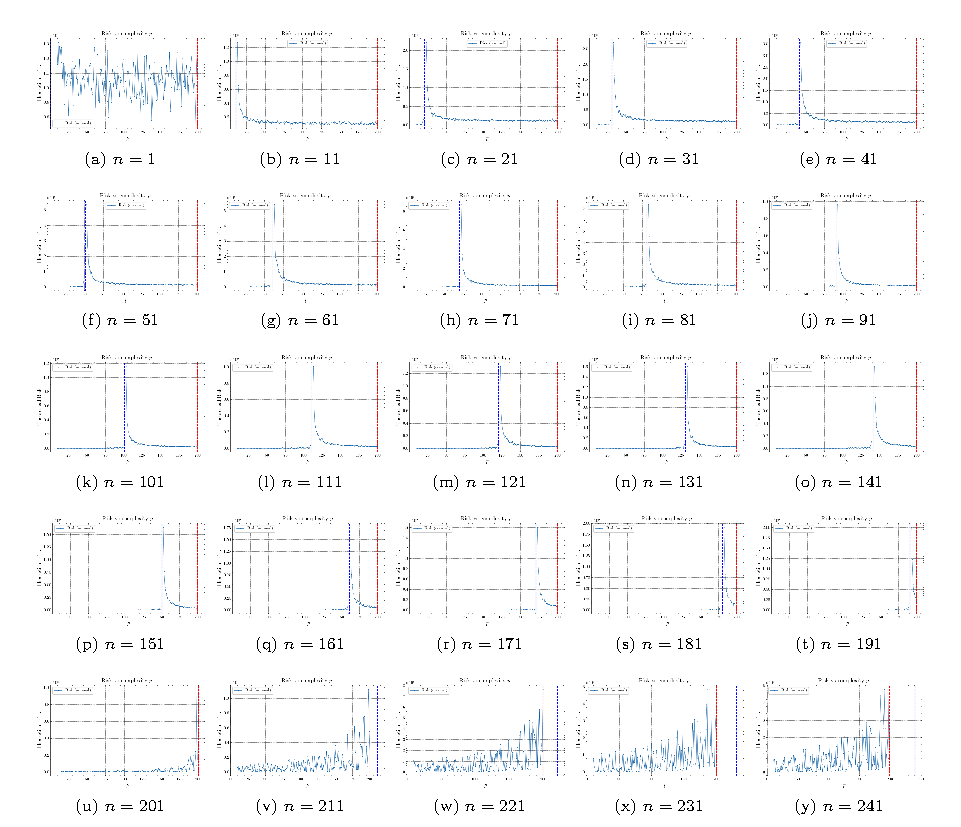
\includegraphics[width=0.8\textwidth]{pdf/linear_gen.pdf}
    \caption{Extension general experimentation, using the prediction made of theorem~\ref{thm:double_descent_lr} for verification. Here, $q=1$ as the general basis case of verification. }
\end{figure}

A design of the above class will require, in general, a much less straightforward implementation than the least square method, at least when it comes to circumstances and case fielding. The previous experimental result was done using a straightforward, single-time calculated theorem. To verify such, we need to adopt the non-zero class in a way that is static of the entire training procedure, and so on, for larger and larger $q$. First, we discuss of the mismatch calculation and thereof taken from the iterative error segmentation. In our cases, we have $h$ and $c$ with \textit{model mismatch}, that is, there might exist certain parameter that $h$ has, but the concept $c$ of its originality does not, and vice versa for the concept model of which the hypothesis does not have, or attain certain parameter of interest. This prompts us to make use of a type of \textbf{penalty} for such case. With respect to the mean square error on parameter, from the perspective of the supervisor, we have two ways to implement this, either of the $\mathsf{truncate}$ or $\mathsf{padding}$ mode. The truncate mode simply calculates parameter expression of those that can be compared. By default, for the learning problem to be consistent of the space, there must be at least one parameter that is not inhibited. Then, 
\begin{equation}
    \mathrm{MSEP}_{\text{truncate}}(h,c) = \frac{1}{k} \sum^{k}_{i=1}(p_{i}-q_{i})^{2}
\end{equation}
For $K=\min(n,m)$ of the overlap, or can be changed to be the set $k=\{(h_{i},c_{i})\}$ of which matches each other. Such can be changed to absolute error, if one does not want to inflate the error measure beyond its distance metric with respect to certain axis. The $\mathsf{padding}$ mode simply takes into account of all missing or surplus information and of the optimization phase. By initialization, from the hypothesis side, all surplus parameters are padded with input $1$. Hence, the measure is defined as 
\begin{equation}\label{eq:parameter_penalty}
    \mathrm{MSEP}_{\text{pad}}(h,c) = \frac{1}{k} \sum^{k}_{i\in k} (p_{i}-q_{i})^{2} + \lambda \left(\frac{1}{n-k}\sum^{n}_{i\not\in k}p_{i}^{2}+ \frac{1}{m-k}\sum^{m}_{i\not\in k}q_{i}^{2}\right)
\end{equation}
The total error then is simply the above error, is simply calculated toward all layers possible or any architectural design parameters. This design will be also used in subsequent testing, including polynomial, in which the effectiveness is enhanced significantly. 



\section{Polynomial models}

\subsection{Structure}

For mathematical analysis and experimental design, we would like to state the current main structure of a polynomial model. Specifically, in such example, we are concerned of the shallow polynomial neural network, of which is stated as such in \cite{arjevani2025geometryoptimizationshallowpolynomial}. Notice that it is defined on the normal Vandermonde basis, where an expression of such polynomial model under Newtonian or Lagrangian basis is not so clear-cut of an analysis. 

\begin{definition}[Shallow polynomial neural network]\label{def:poly_structure1}
    A shallow polynomial is a neural network of one layer that are functions $f_{\mathcal W}$, defined such as:
$\mathbb R^d \rightarrow \mathbb{R}$ of the form
\begin{equation}\label{eq:network_model} 
    \begin{split}
        &f_{\mathcal W}(x) = \sum_{i=1}^r
\alpha_{i} (w_i \cdot x)^d,\\  
&\mathcal W = (\alpha,w_1,\ldots,w_k) \in
\mathbb{R}^r \times (\mathbb{R}^{n})^k,
    \end{split}
\end{equation} 
where $d \in \mathbb{N}$.
\end{definition}

A modification is then available, in which we simply add $b(\cdot)$ for random initialization process. We note that this introduces certain flexibility to the model initial interpolation curvature.   
\begin{definition}[Polynomial neural network, general]\label{def:poly_model_test}
    The polynomial network based on Model~\ref{def:poly_structure1} is modified as 
    \begin{equation}
        f_{\Theta}(x) = \sum_{i=1}^{d} \theta_i \left( \mathbf{w}^\top x \right)^i + b,
    \end{equation}
    where $\Theta = (\{\theta_{i}\},\{w_{k}\},b)$.
\end{definition}

From this, we can state the model within a testing scenario listed as such, to fully capture the structural foundation of the related testing model class. For the notion of complexity, naively, we employ two kinds of complexity measure. First is the usual complexity measure via parameter counts. Second, is the expressive complexity on the basis of the linear transformation space. That is, an expressive complexity that take into account the fact that $\mathcal{O}(wx^{n})$ will always be stronger than $\mathcal{O}(wx^{n-1})$ for $x>1$. All of which can be contained in a singular expression, as seen in definition~\ref{def:pec}. However, we would have to analyse what is happening inside the metric itself. The model itself is illustrated in Figure~\ref{fig:plm}.

\begin{table*}
  \centering
  \footnotesize
  \begin{threeparttable}
    \caption{Controllable parameters and hyperparameters for polynomial class analysis}
    \label{tab:polynomial_test}
    % three columns: adaptive widths
    \begin{tabularx}{\textwidth}{ L{0.25\textwidth}
                                     L{0.2\textwidth}
                                     >{\RaggedRight\arraybackslash}X }
      \toprule
      \textbf{Information} & \textbf{Notation} & \textbf{Details} \\
      \midrule
      Hypothesis model
        & $h[\mathcal{W}_{h},\mathbf{H}_{h}]\in \mathcal{H}$
        & Hypothesis model. For simplicity, it contains $\mathcal{W}$ as the configuration parameter set, and $\mathbf{H}$ the fixed hyperparameters \\
      \addlinespace[1pt]
      Concept model
        & $c[\mathcal{W}_{c},\mathbf{H}_{c}]\in \mathcal{C}$
        & Concept or target model. Similar configuration as the hypothesis model \\
      \addlinespace[1pt]
      Complexity measure(s)
        & $\{\mathbb{C}(\cdot)\}$
        & Set of complexity measure of choice for any arbitrary model taken in. \\
      \addlinespace[1pt]
      Sample count
        & $m$
        & The number of sample available for hypothesis model of $c$, for $m=|\mathcal{S}|$ dataset\\
      \addlinespace[1pt]
      Hypothesis dimension (hyperparameter)
        & $[d_{h}]$
        & An explicit hyperparameter contains the list of all in-testing polynomial degree for the hypothesis model. \\
      \addlinespace[1pt]
      Concept dimension (hyperparameter)
        & $d_{c}$
        & An explicit hyperparameter of the concept's true dimension. Theorized such that $d_{c}=d_{h,i}$ for arbitrary $i$ will reduce to possible low-error problem.\\
      \addlinespace[1pt]
      Data noise
        & $\epsilon_{\mathcal{S}}$
        & Dataset-wide noise with relative strength to the value of the sample point. This is to reduce vanishing noise with higher-degree polynomial sample points. \\
      \addlinespace[1pt]
      Learning parameters
        & $\mathrm{epoch}, lr, \mathrm{bs}$
        & Two main parameters for gradient-descent, iterative-based algorithm - the epoch, the learning rate, and the batch size.\\
      \bottomrule
    \end{tabularx}

    \begin{tablenotes}
      \footnotesize
      \item[] \textbf{Notes:} We output to $\{\mathbb{E}[\ell]\}$ as the expected value of the error measure on $h,c$. There are a few things possible, but under approximation setting, we use MSE-on-parameter and MSE-on-prediction for two different insights: internal representation and external representation. 
    \end{tablenotes}
  \end{threeparttable}
\end{table*}

\begin{figure}[htb]
    \centering
    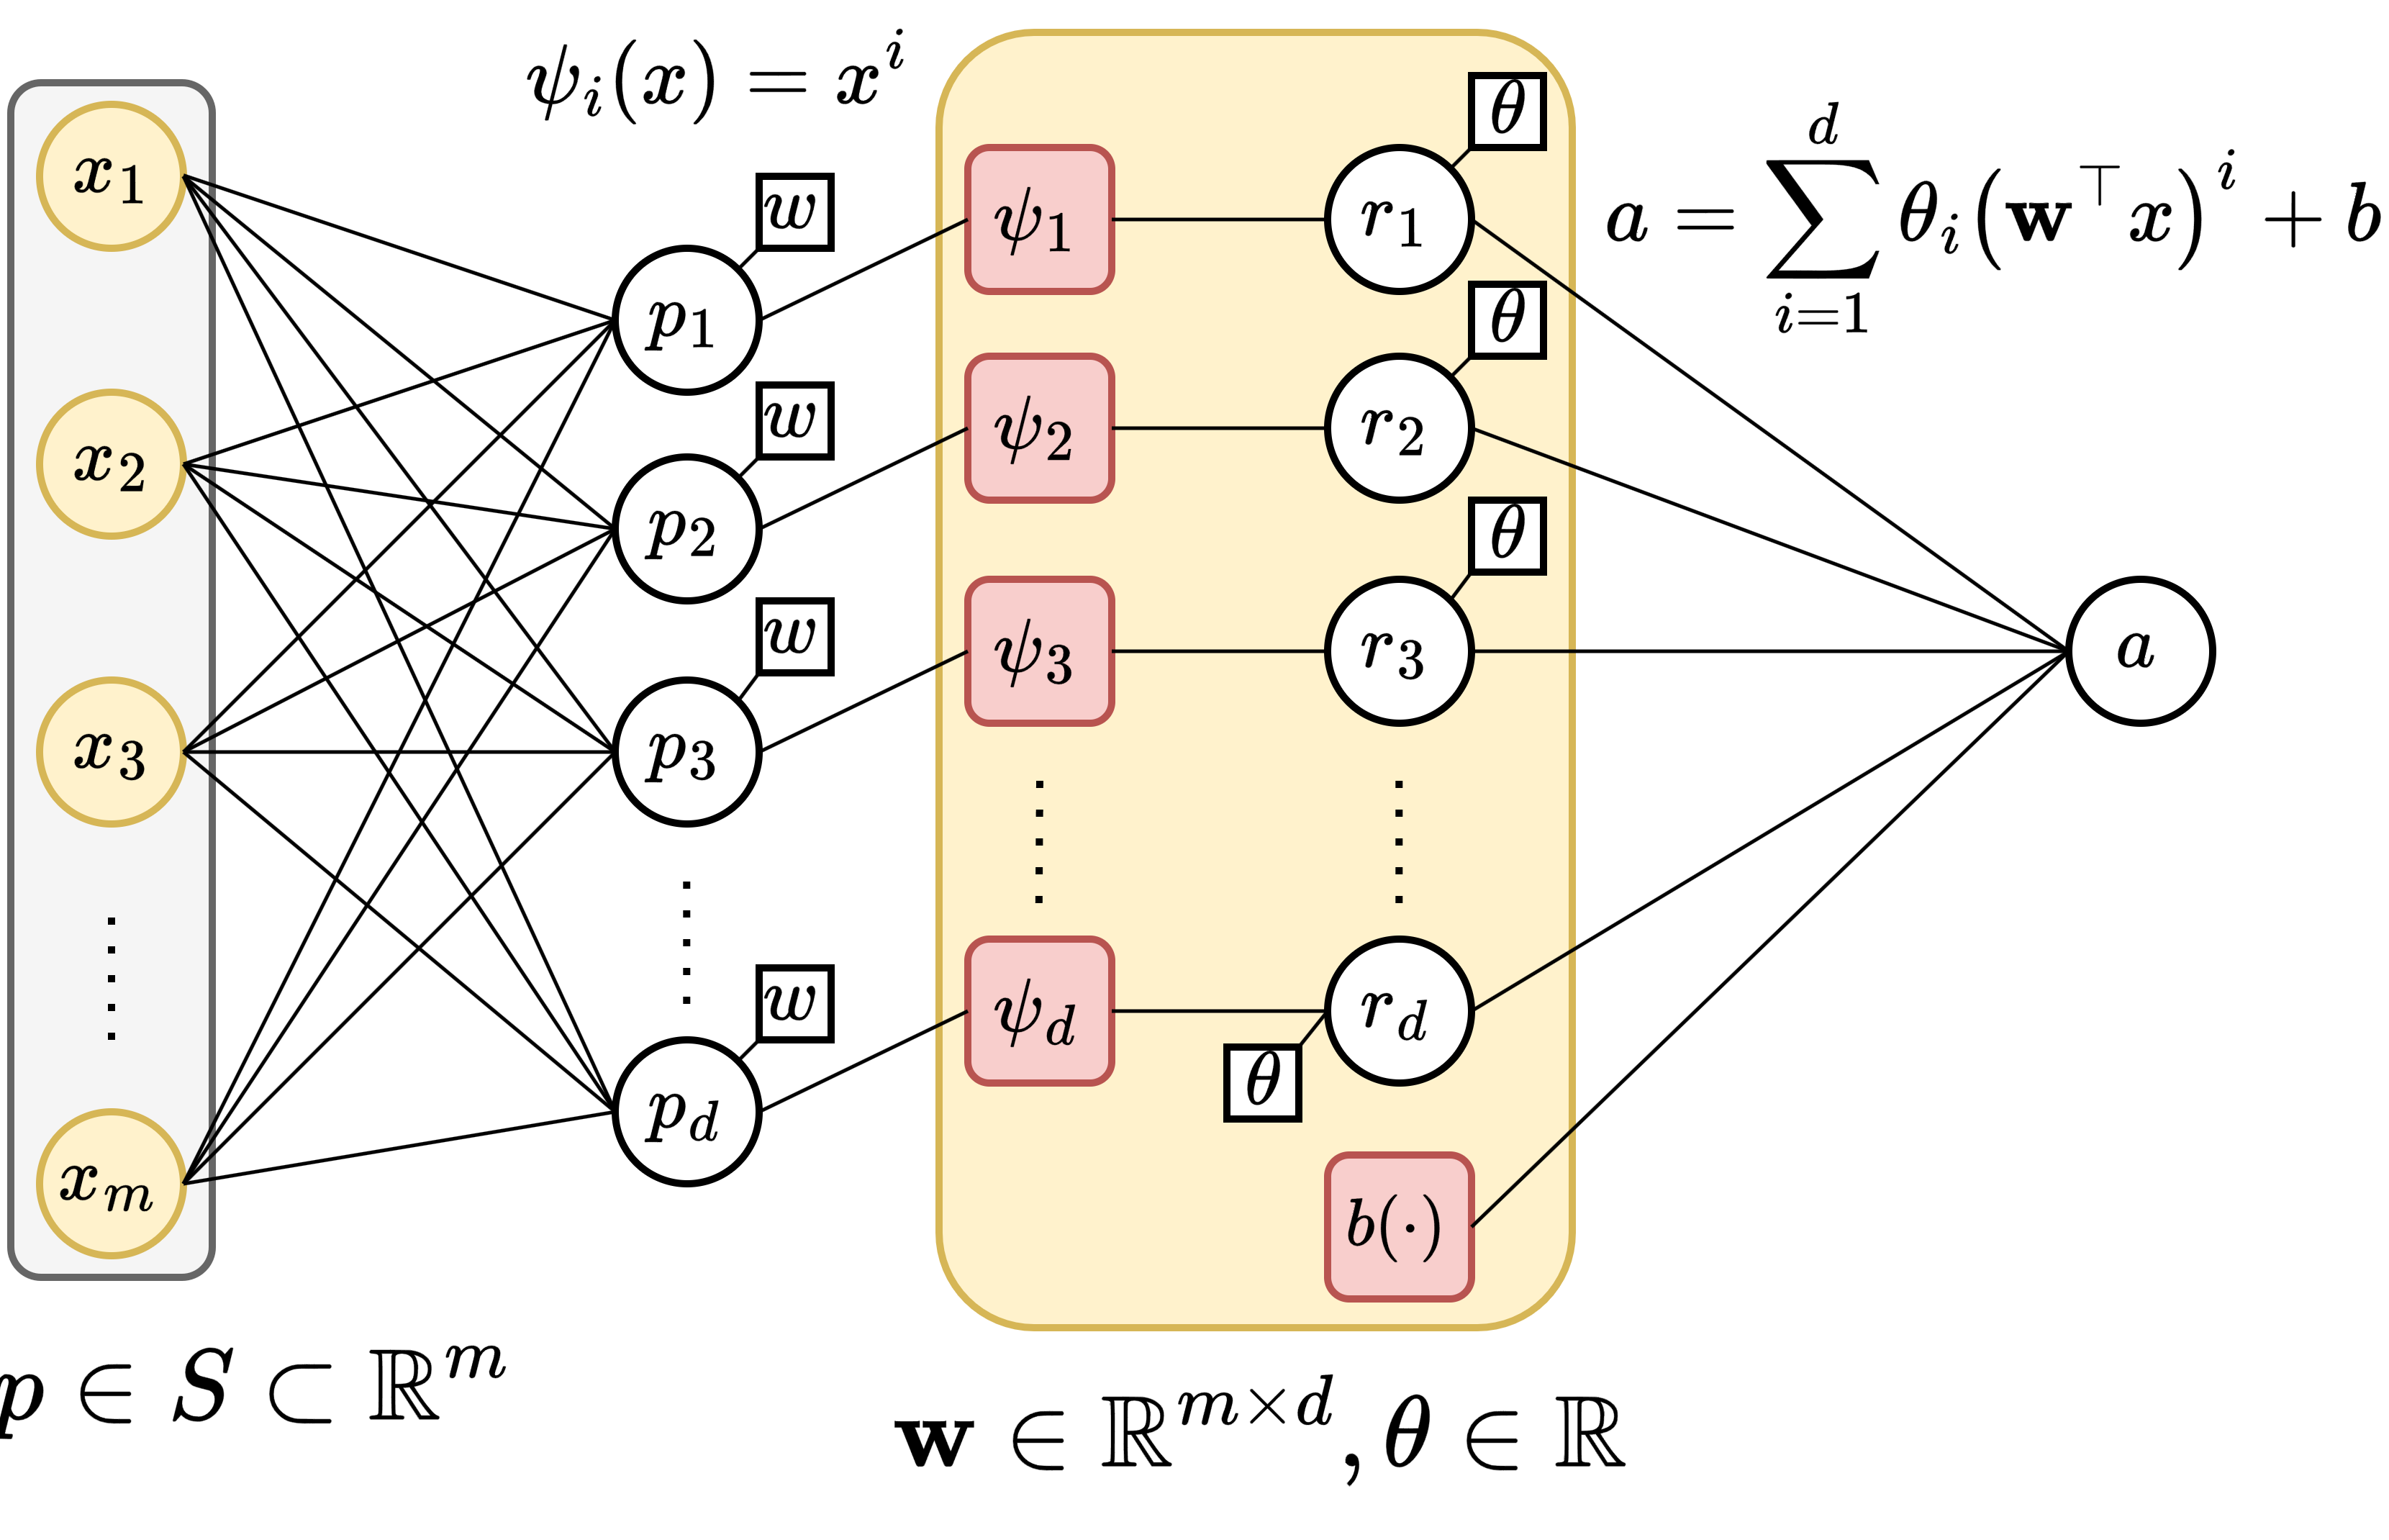
\includegraphics[width=0.5\linewidth]{media/diagram_poly_model.png}
    \caption{Illustration of polynomial model in definition~\ref{def:poly_model_test}.}
    \label{fig:plm}
\end{figure}

In the equation for expressive complexity, the first term is the normalized linear parameters $\theta_{i}$ fixing and controlling the shift of the polynomial inning parameter, the second term is the sum of weight-aware complexity with degree factor, and the degree factor over operating range $||x_{max}-x_{min}||$ of the dataset, for the degree complexity. The final term is the last weight-aware complexity for the dominating degree $n$ of the polynomial function. Let us begin with the gauge on coefficient norm, i.e. the term $||\alpha_{d}||+1$. Here, we set $1$ as baseline, and the arbitrary norm on $\alpha$ there coefficient effect. The terms coefficient in this expression matters because, for a function $f:[a,b]\to\mathbb{R}$, the Lipschitz constant $L$ for polynomial $f$ goes by 
\begin{align}
L_{p} 
&= \sup_{x \neq y} \frac{|f(x) - f(y)|}{|x - y|} \\
&= \sup_{x \neq y} \frac{|f_{\Theta}(x) - f_{\Theta}(y)|}{|x - y|} \\
&\leq \sup_{x \in [a,b]} \left\lVert f_{\Theta}'(x) \right\rVert_{2} \\
&= \sup_{x \in [a,b]} \left\lVert \sum_{i=1}^{d} i\,\theta_i\,(\mathbf{w}^\top x)^{\,i-1}\,\mathbf{w} \right\rVert_{2} \\
&\le \lVert \mathbf{w} \rVert_{2}\; \sup_{x \in [a,b]} \sum_{i=1}^{d} i\,|\theta_i|\,|\mathbf{w}^\top x|^{\,i-1} \\
&\le \lVert \mathbf{w} \rVert_{2}\; \sum_{i=1}^{d} i\,|\theta_i|\,\max\!\big\{ |\mathbf{w}^\top a|,\,|\mathbf{w}^\top b| \big\}^{\,i-1}.
\end{align}


Where we note that $f_{\Theta}(x)=\sum_{i=1}^{d} \theta_i \left( \mathbf{w}^\top x \right)^i + b$, and $||\mathbf{w}||_{2}$ is the Euclidean $\ell^{2}$ norm. The magnitude of $f_{\Theta}'(x)$ depends directly on the coefficient size $\alpha_{i}$, and also on how big is $x$ on the domain. All of this mean for large expression and value range on $f_{\Theta}$, the Lipschitz constant of that model is accordingly large. Defining $\alpha$-norm that way is a cheap proxy for Lipschitz constant, since it gauges stability, and rate of change of the functional expression itself. 

\begin{definition}[Polynomial expressive complexity]\label{def:pec}
    For $x>1$ or $\mathbf{x}_{i}>1$ of $\mathbf{x}\in\mathbb{R}^{n}$ as input. Denote the polynomial class as $\mathcal{P}_{n}$ of their highest degree $n$, then we define the total expressive complexity of $p\in \mathcal{P}_{n}$ as followed.
\begin{equation}
    \begin{split}
        &\mathbb{C}_{E}(p)\\
& \quad = \mathbb{E}\!\Bigg[
\lVert \alpha \rVert_{d} + 1\\
& \quad + \frac{\sum_{i\in S\setminus\{p_{n}\}} w_i\,i}{\|p\|-p_{n}}\\
&\quad + \frac{1}{||\overline{x}-\underline{x}||}\!\left(
\frac{\sum_{i\in S} i}{\lVert p\rVert } + w_{n}n
\right)
\Bigg],
    \end{split}
\end{equation}
    where $S=\{p_{j}\}$, $||p||$ denotes the amount of different degree separable terms and $||x_{max}-x_{min}||$ is the observable range of the dataset. 
\end{definition}

\subsection{Scenario schema}
The scenario schema will be as followed. The following set of parameters are required for controlling the testing case, aside from different system measures. For parameter error, we reuse equation from Definition~\ref{def:pec} but with degree aware terms. This is covered in Table~\ref{tab:polynomial_test}.

We note a few problems with both interpolation interpretation and polynomial regression of higher-degree terms. Firstly, is the intrinsic interpolation error and numerical, software issue error. Higher degree polynomial can be represented as solving for a wide Vandermonde system of $n$ degrees for $m$ sample points. Using monomial basis for interpolation, either for soft interpolation also exhibits instability and numerical garbage within the operations, as indicated by \cite{Shen_2025}. They can also be a potential source of double descent, as the majority of models tested around this range are not coded effectively for handling large data operations as such, and artifacts from such choices might be taken as the indication of double descent in some particular cases. 

Aside from it, and aside from the fully-connected case, we have the particular testing scenario that can be expected of the ease of implementation. First, is the mundane implementation that is of gradually increasing degree mismatch. That is, for polynomial of $h_{p}$ and $c_{p}$, one requires only $d_{h}$ and $d_{c}$ to figure out the structure as there will exist exactly $d+1$ with the constant term, terms of which of finite many degrees. The second case is where for $p$ chosen randomly, such that aside from such $p$ entry, then the other degree or nodes of input are simply scattered dependent nodes, linear algebraically. That is, for a uniformly constructed $d$-degree network, choose at random $p$ particular degree to be fixed, while the other of $d-p$ are assigned randomly of belonging to some $p_{i}\in \{p\}$ nodes given the random choice on $p$ above. Linearly algebraically, scattered and dependent nodes then mean for example, node $4$ might use node $35$'s degree, and vice versa (if they were both non-fixed). The dependency structure is deliberately randomized rather than organized. For overparameterized case, we simply design the hypothesis by the following line of justification. For a mapping $\mathbb{R}^{d}\to\mathbb{R}$, the mapping $\mathbb{R}^{d+n}\to \mathbb{R}$ for $n= 1$ requires additional information, since the source provision does not contain information to handle additional $n$ dimensional input. Hence, we design it the following. For the hypothesis $h$, such unit of which does not fit to the original input space, the \textit{internal input space} that $h$ `hypothesize' contains, for the other $n$ entries, $q\leq d$ per unit input. That is, each input of $n$ overparameterized case receives at random, $q$ inputs can be received, for example, $w_{n1}x_{j}+w_{n2}x_{k}$ for $k,j$ specific input numbering. By the simplicity argument, then $q=1$ for the simplest case. However, this creates a skewed polynomial network, of which informally, the provided structural bias or additional information, is the fact that there exists overparameterization. To prevent this, instead, the final case considers the most general structure --- for each unit, each one can take $q$ inputs controlled as hyperparameter of the network, then the set $\{p\}$ of chosen degree influence their degree choice, and is uniform if the sampling process it is not included. 

\subsection{Procedure}

The procedure for making the observation space, i.e. the most important one, will be as followed. Specify finite $|\mathbf{X}|_{\mathbb{E}}$ denotation for admissible value region (if multivariate polynomial) of the observables' intended context coverage. Second, initialize \textbf{random shutdown} choice of the Oracle with arbitrary structure, in which this case we simply use polynomial component. Generate portion of $1$ for the true oracle without shutdown, and introduce a mixture as followed: for $k$ shutdown sequence, more severe than another, assign choice of choosing such data into the final dataset by Poisson distribution on $\lambda^{k}e^{-k}/(k!)$ of arbitrary $\lambda\in\mathbb{R}_{+}$. For fixture, we assume $\lambda=0.2$. Then finally, sample on the generated shutdown corruption, and add intrinsic noise, for $\epsilon_{i\leq m}\sim \mathcal{N}(1,\sigma^{2})$ tuneable for intrinsic noise change, and thus finish the initialization of the observation space.

\clearpage


\section{Graph Neural Network (GNN) - \cite{shi2024homophilymodulatesdoubledescent}}
To confirm and observe particular insights on the problem, experimentally, we focus more on the results given by the analysis on a particular type of neural network, the graph neural network (GNN). However, preliminary experiments are also needed, for example, with various complexity and function class, though most of them are algorithm based on ERM, which typically can be called derivation of gradient descent. 

According to major literature, for example, \cite{shi2024homophilymodulatesdoubledescent}, double descent is absent usually in GNN, for example, GCN networks. However, in fact, it is relatively unstable, as for certain papers and researches point out its existence and variation of it being ubiquitous to the network, some reports none of such occurrence in their experiments. Thereby, our first strategy would be to encounter this absence, and the way to force it to exhibit itself, if the phenomenon is perceived non-existent. In experiments by \cite{shi2024homophilymodulatesdoubledescent,buschjager_generalized_2020}, we know that graph network are inherently sensitive to data configuration. The graph MPNN in \cite{GRP_Hamilton}, for example, depends heavily on the configuration of data to present its neighbourhood aggregation for each layer. However, we would like to first claim the dichotomy of bias-variance holds for it to be presented as the first interpolation point.

We would use, and utilizes a hybrid setting between MPNN, GCN and GAN (attention network), to configure out network in itself. However, heterogeneous network - either consists of only MPNN or GCN layers, is somewhat preferred for ease of analysis, and potency of experimental learning control. Because double descent lies between the concept of test error and training error, either supervised or semi-supervised would be used. According to \cite{shi2024homophilymodulatesdoubledescent}, semi-supervised setting gives better flexibility and overall 'range' of operation. Other than GNN, certain more abstract, 'vanilla' neural network formalism as specified in the above section treatment will also be conducted, in a supplementary manner. 

\subsection{Methodolody}

Because of the irregularity in the statement that GNN does not exhibit any phenomena that is related to double descent \cite{shi2024homophilymodulatesdoubledescent}, we would be investigating this phenomenon the most. This particularly means that a lot of our focus will be to analyse the GNN network by itself. 

\subsubsection{Quick introduction to graph theory}

A \textbf{graph} $G$ is a 2-tuple $(V,E)$ where $V$ is the set of \textbf{vertices}(or nodes) and $E$ is the set of \textbf{edges}. The set $ne[n]$ stands for the neighbour of vertex $n$, while $co[n]$ is the set of edges that have $n$ as vertex. Edge is often denoted by $(u,v)$ for vertices $u$ and $v$. We said that $(u,v)$ \textbf{joins} $u$ and $v$, and it can be directed or undirected. A graph is called a \textit{directed graph} if all edges are direct or \textit{undirected graph} if all edges are \textit{undirected}. The \textbf{degree} of vertices $v$, denoted by $d(v)$, is $t$ number of edges connected with $v$.
The graph data can be loosely (not specifically in cases) as followed. Let $\mathcal{G}=(\mathcal{V},\mathcal{E},\mathcal{W})$ be a graph, where $\mathcal{V}=\{1,\dots,n\}$ is the set of nodes, $\mathcal{E}=\{1,\dots,M\}\subseteq \mathcal{N}\times \mathcal{N}$ is the set of edges, and $\mathcal{W}: \mathcal{E}\to \mathbb{R}$ is the edge's weight function. There is also the optional weight $\mathcal{W}': \mathcal{V}\to \mathbb{R}$ for each vertex. In this case, it is for certain problem like TVP, where all cities have certain properties for the path. We say that a data sample $\mathbf{x}$ is a graph data, if its entries are related through the graph $\mathcal{G}$. 

Our 2-tuple $(V,E)$ and the collection of all such tuple forms a group of \textit{simple graph} (undirected) and \textit{directed graph}, where the only change is that $(u,v)\neq (v,u)$ for any given edge on a graph. From such, a typical setting, if we are to apply a machine learning setting on graph-theoretical problems, can be described as the following

%\begin{definition}[Graph-theoretical edge learning]
%    Given a graph $G(V,E,\psi_{E})$ for $\psi_{E}$ the edge proprietary classification, there exists an encoding space %$\mathsf{ENC}(G)$ that the graph lives in, and a function $\phi: (E,\psi_{E})\to (E',\psi_{E}')$ such that to change %the configuration of the connector space. The \textbf{learning problem} is for a learner $\mathcal{L}$ to learn a %function $\phi$ that is appropriate of the intended use case, such that for any given data $D(V^{*},\odot)$, either:
%    \begin{enumerate}
%        \item Assign $E^{*}$ and transform to $\psi_{E}^{*}$. 
%        \item For existing $E^{*}$, transform to $\psi^{*}_{E}$. 
%    \end{enumerate}
%    All within the marginal error evaluation of $L$. 
%\end{definition}



Much information can be packed on a graph. Typically, the graph $\mathcal{G}= (\mathcal{V},\mathcal{E},\mathcal{M})$ will contains node information and edge information. Edge information can be the path-only, or weight-specific, that is, there exists for an edge $(u,v)$ a property $\phi_{uv}\in [0,1]$ acting like a weight to gauge a walk on the graph. This can also be used for the \textit{distance measure} of a graph, for such graph being represented with values per position, that is, each node/vertice has position, and similarly there exists arbitrary distance $\lvert (u,v)\rvert$ between $u$ and $v$. Any space that encode a graph's information in such way is called an \textbf{embedding space}. For node information, connections to other nodes are one type of information; however, it also retains its own properties, typically inferred through the \textit{node embedding space} which contains features of a node and the graph itself. There are a few restrictions of such embedding space, such as to define the node embedding space to be of the same shape $n$, to avoid `edge cases' in the process. 

The reason for choosing an encoding can be justified as followed. Typically, graphs can be classified and categorized into a specific type of data representation, called \textit{non-Euclidean data}. More specifically, there exists a topological space encapsulating the graph, but exists no fundamental measure on such topological space housing it. For example, there exists no notion of a \textit{discrete distance} on a graph, but only the induced notion of \textit{graph distance} by counting the shortest path from one node to another in a specific graph. Because machine learning works on the assumption that the space of the system gives \textit{measurable space}, a natural response is to encode the system into an encoding space of arbitrary meaning. One, for example, simple encoding is the degree map, where nodes are mapped into an $n\times n$ matrix of nodes and valued by the number of neighbour they have. 

This type of encoding then creates, for each graph, a versatiel number of arbitrary properties space they can have, stacked on each other. Typically, for a hypothesis $h$ to work on a graph $\mathcal{G}$, then it will have two main targets that act directly on the graph, as illustrated in Illustration~\ref{fig:graphdecom}.
\begin{figure}[htb]
    \centering
    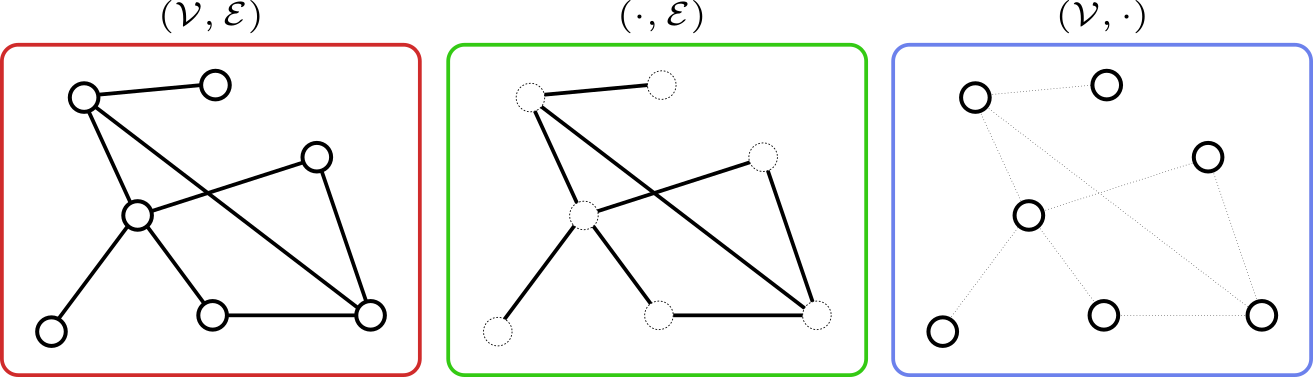
\includegraphics[width=0.7\textwidth]{media/img/graphdecom.png}
    \caption{Illustrative decomposition of the graph on its simplexes edges and vertices: Each of the decomposed space $\mathcal{V}$ and $\mathcal{E}$ can be encoded separately to their own ordeal, for example, of the edge connection through incident matrix.}
    \label{fig:graphdecom}
\end{figure}
There are many ways or aspect of a graph to be `extracted' from the graph features itself. Classically, this is done using feature engineering (\cite{GRP_Hamilton}) and hence the learner is also configured to utilize such features. Nowadays, it is mostly abstracted into an arbitrary representation space of the graph encoding, used in neural network architectures (\cite{Oono2020Graph,lopushanskyy2024graphneuralnetworksgraph,Scar04,GRP_Hamilton}). The only different between the classical encoding and the deep learning encoding is on the arbitrary properties of deep learning encoder, of which the transformed feature might not be well-defined feature engineering as the classical case. 

This prompts two types of main learning targets: either to have the hypothesis $h$ to learn the edge connections and properties, or to learn on the vertices/node. They are, however, not separated, as to learn about which connections $e\in \mathcal{E}$ to make between two nodes requires information about the general graph's node itself, to predict which node would be connected under obscured information (removing edges). So, there are: 
\begin{itemize}[topsep=0pt,noitemsep]
    \item \textbf{Edge reconstruction}: predict if there exists an edge at an arbitrary segment of the graph, for example, between $u,v\in \mathcal{V}$. 
    \item \textbf{Edge classification}: An edge $e\in \mathcal{E}$ is endowed a label, and we will then try to classify it based on the actions, or properties it has on the graph. 
    \item \textbf{Node classification}: Classify a node $v\in \mathcal{V}$ of certain class of labels. 
    \item \textbf{Node regression}: Estimate values of certain nodes. In turns, it might also be used for ranking certain nodes based of specific criteria. 
\end{itemize}
It is helpful to see that a graph can also be classified into two more main archetypes, based off their actions: either \textbf{static}, where the node and edges remains the same, or \textit{dynamic}, where deletion of nodes and edges and vice versa are taken into account. The problem revolving a dynamically changing graph (as more prominent in real-life cases) is resolved using temporal methods for graph learning (\cite{rossi2020temporalgraphnetworksdeep}), however, it is much more difficult to analyse, and hence we would restrict ourselves in the case of static graph analysis. 

We then state our problems in regard. 

\begin{definition}[Graph learning problem]
    Given a graph $\mathcal{G}(\mathcal{V},\mathcal{E})$, for any type of graph-theoretical subtype (multigraph, digraph, etc.) by $m$ contraints. There then exist two topologies: the \textbf{graph-theoretical topology} of connections and nodes appearances, and the \textbf{encoded topology} of various measured properties for all $v\in \mathcal{V}, e\in \mathcal{E}$, denoted by $(\phi_{G},\phi_{E})$. A hypothesis $h\in \mathcal{H}$ is then tasked to learn its own encoding, or loosely speaking \textbf{interpretation} of the hypothesis about $\mathcal{G}$ based on the topological space given by $\mathcal{G}$, and use it to target or solve problems related to both $\phi_{G}$ and $\phi_{E}$. 
\end{definition}

From this, we might derive various problems setting as it is, and considering the set $\{\phi\}$ of encoding intrinsic to the graph. 

\subsubsection{Graph Neural Network}

We target the graph neural network structure (GNN), specifically a neural network implementation for solving graph data problems. A more detailed description can follow from \cite{GRP_Hamilton,Scar04}. Typically, graph neural network (\cite{Scar04,Veli_kovi__2023,tanis2024introductiongraphneuralnetworks,lopushanskyy2024graphneuralnetworksgraph}) follows the instruction flow of the \textit{encoder-decoder} architecture. A GNN is formulated and structured by analysing a graph data system by conceptually apply a \textit{neighbour-dependent} neural input arrangement on top of the data. That is, in principle, it reserves on its own a particular extractor and modifiers on the graph interpretation itself, through its layers. 

Structurally, the description of a GNN is defined by the overall \textit{message-passing neural network} (MPNN), defined by (\cite{pyg_docs,Fey/Lenssen/2019}): 

\begin{equation}
    \mathbf{x}_i^{(k)} = \gamma^{(k)} \left( \mathbf{x}_i^{(k-1)}, \bigoplus_{j \in \mathcal{N}(i)} \, \phi^{(k)}\left(\mathbf{x}_i^{(k-1)}, \mathbf{x}_j^{(k-1)},\mathbf{e}_{j,i}\right) \right),
\end{equation}

for $\bigoplus$ the differentiable, permutation invariant function, usually called the aggregator, $\mathbf{x}^{(k-1)}_i \in \mathbb{R}^F$ the node features of node $i$ in passing layer $k-1$, $\mathbf{e}_{j,i} \in \mathbb{R}^D$ the optional edge features from node $j$ to node $i$. Additionally, $\gamma$ denotes the nonlinearity differentiable function (usually ReLU, or sigmoid) $\phi$ denote the MLP layer accompanied They are often called the \textbf{updater} and the \textbf{messenger}, respectively. A simplified example of this structure in \cite{Scar04,GRP_Hamilton} as 
\begin{equation}
    \mathbf{x}_i^{(k)} = \sigma \left( \mathbf{W}_{\mathrm{self}}^{(k)} \mathbf{x}_i^{(k-1)} +  \mathbf{W}_{\mathrm{neigh}}^{(k)} \sum_{v\in \mathcal{N}(i)} \mathbf{x}_v^{(k-1)} + \mathbf{b}^{(k)} \right)
\end{equation}

where $\mathbf{W}_{\mathrm{self}}^{(k)}, \mathbf{W}_{\mathrm{neigh}}^{(k)}$ are trainable parameter matrices, and $\sigma$ denotes an elementwise nonlinearity, and an optional bias term $\mathbf{b}^{(k)}$. Different flavours of the differentiable aggregator create the \textit{graph convolutional networks} (GCNs), defined by: 
\begin{equation}
    \mathbf{x}_i^{(k)} = \sigma \left( \mathbf{W}^{(k)} \sum_{v\in \mathcal{N}(i)\cup \{i\}} \frac{\mathbf{x}_{v}}{\sqrt{\lvert \mathcal{N}(i)\rvert \lvert \mathcal{N}(v)\rvert }} \right)
\end{equation}

A somewhat popular approach is to apply attentional layer and weights to facilitate neighbourhood attention, which is called graph attention network.

\begin{figure}[htb]
    \centering
    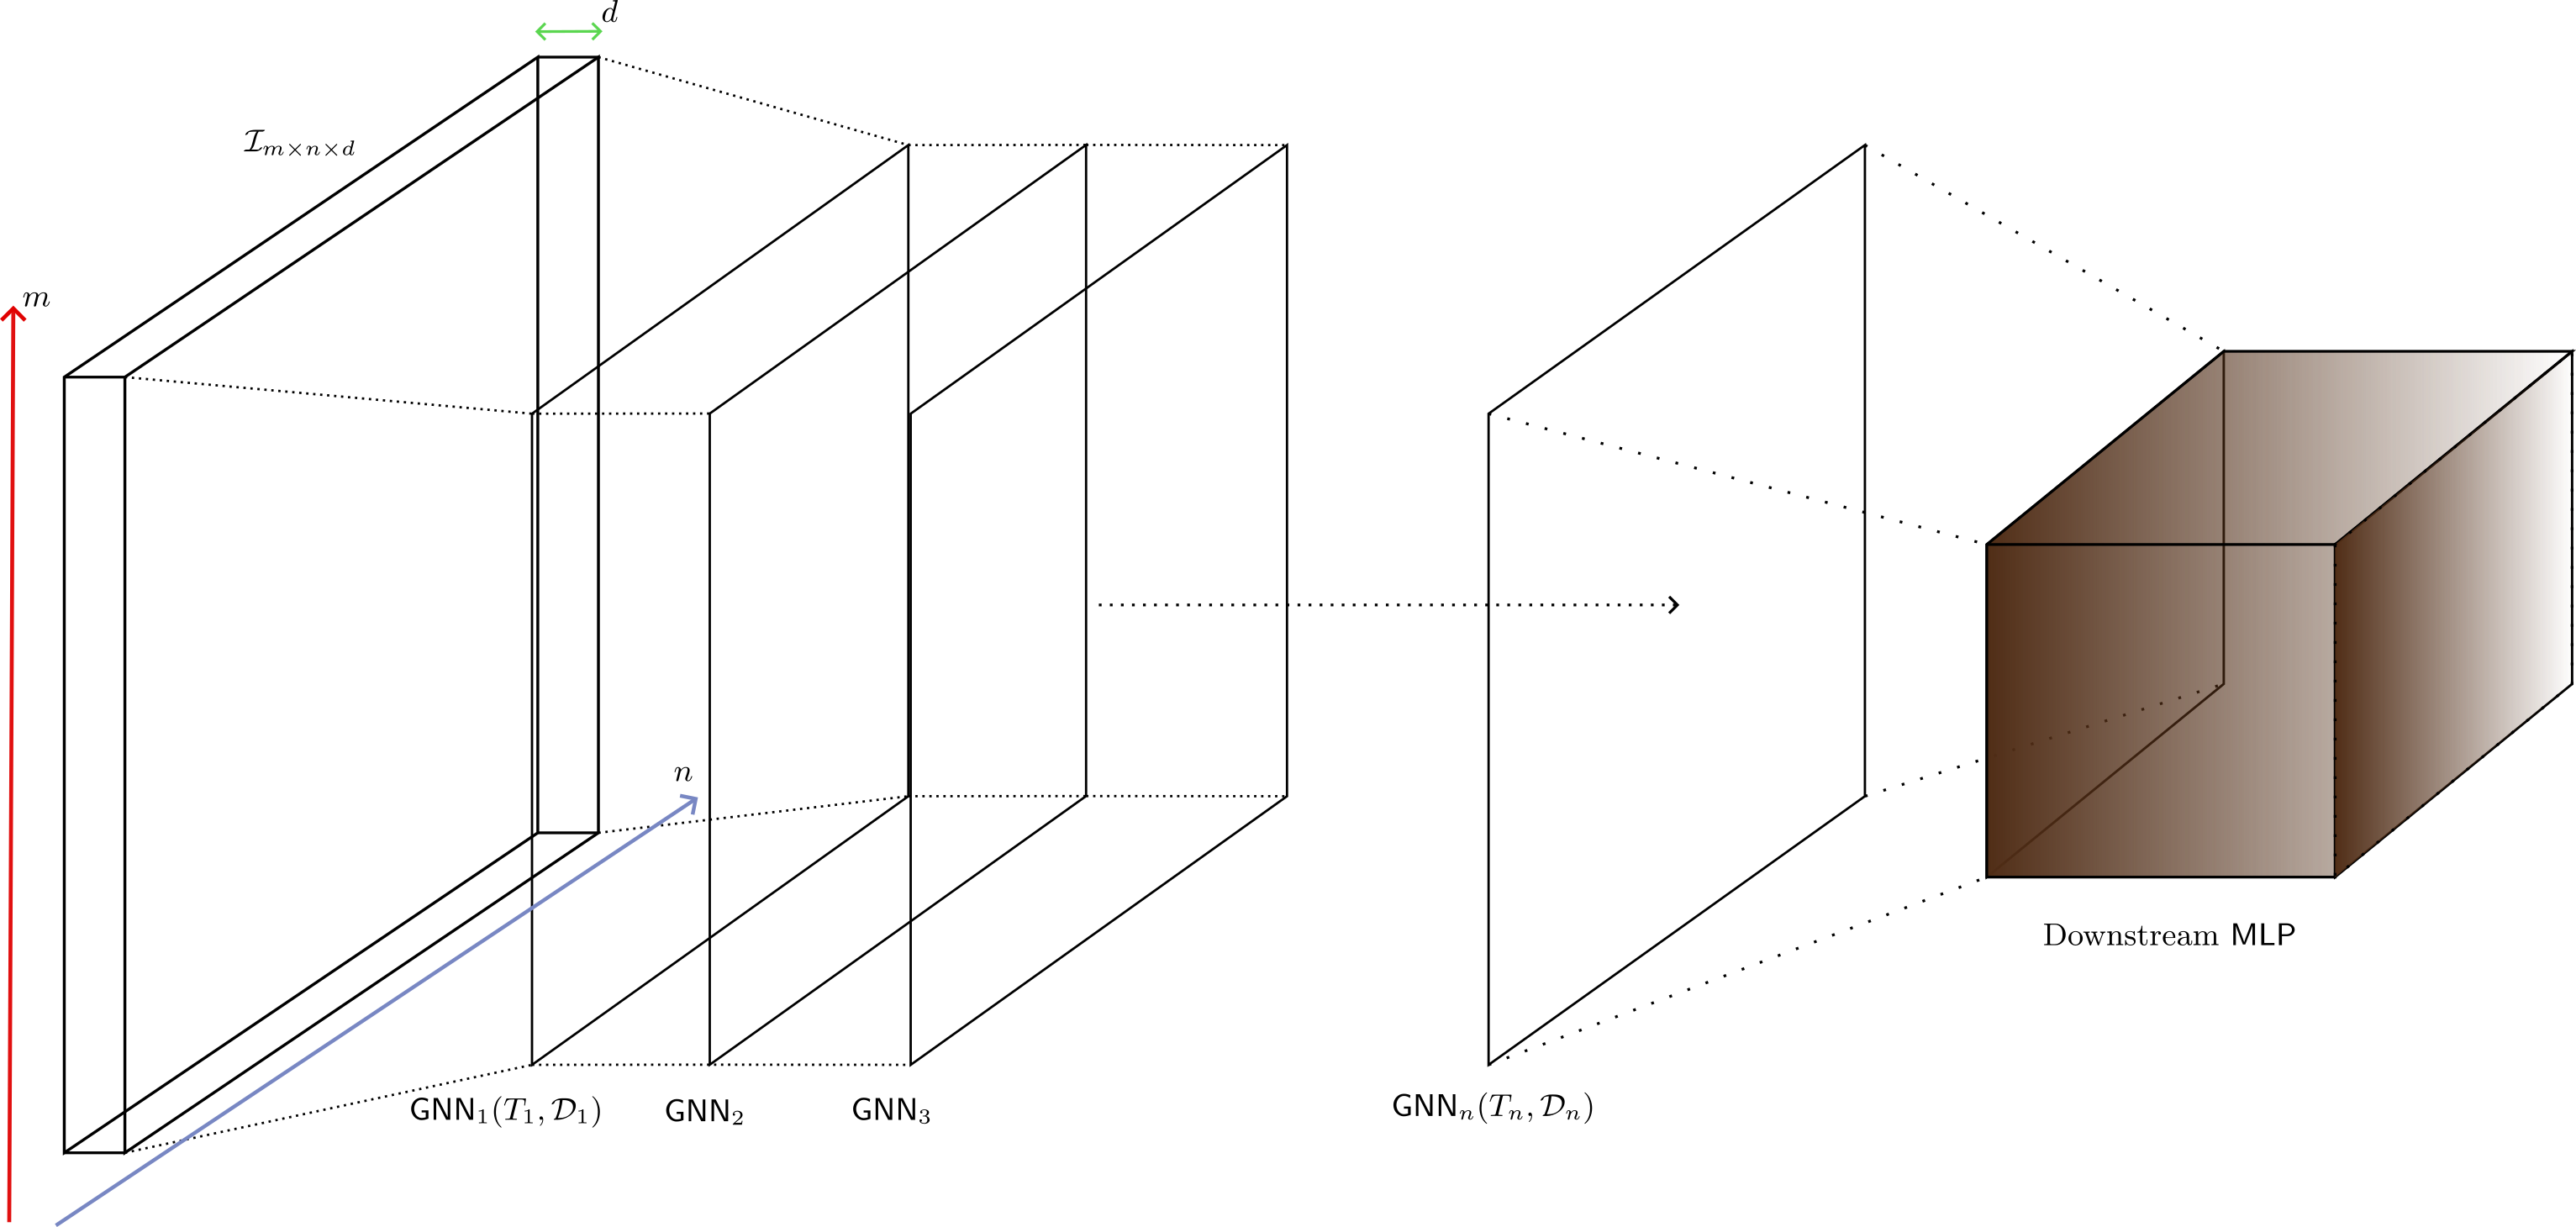
\includegraphics[width=0.8\textwidth]{img/What.png}
    \caption{A conceptual illustration on the running flow of an $n$-layer GNN on particular structure of interest. Note that the data section itself has particular embedding structure on its own.}
\end{figure}

As noted by \cite{GRP_Hamilton}, node features are often required to be inputted into the GNN. Usually, this is of the form $\mathbf{x}_{u}$ for all $u\in \mathcal{V}$. The same can be said for edge in specific tasks required of them. However, if there are no sufficient node representation possible in the first glance, then we can use node/edge statistics as classical techniques. 

\begin{figure}[htb]
    \centering
    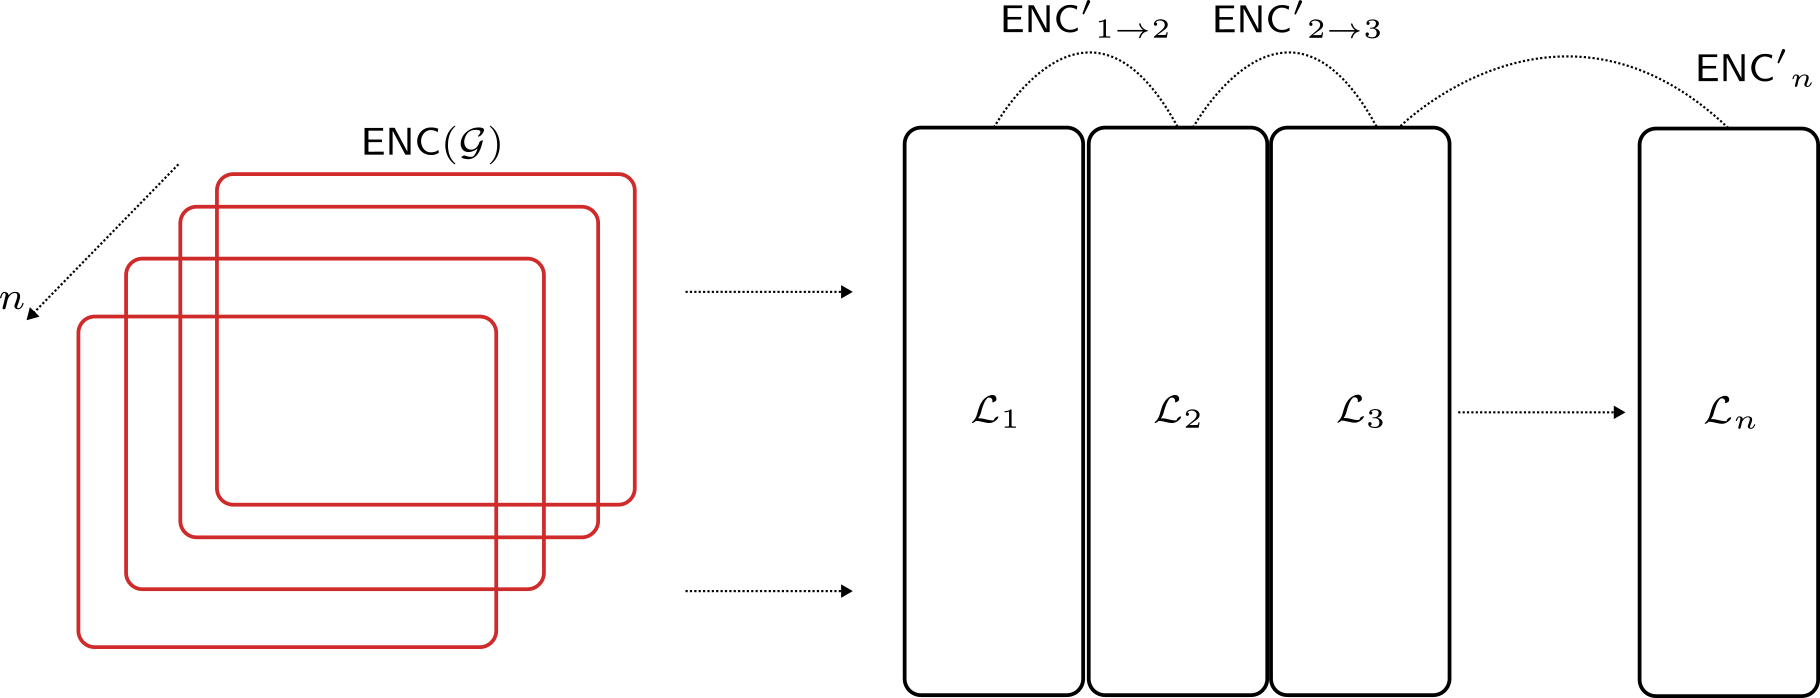
\includegraphics[width=0.8\textwidth]{media/img/gnn_encoding.png}
    \caption{Encoding space and the change of encoding inbetween a static graph (or snapshot-wise) GNN. The encoding space is warped toward arbitrary notions inside a GNN, to the point that after certain layers of processing, the encoding outputs different from expected encoding space (native to the model, not to the designer), though there might be universal notions preserved, like the degree of node represented in a different way.}
\end{figure}

A GNN is, when fitting into the framework of learning system and modeling, is a feature mask generation and adaptation mechanism of the modelling pipeline. What this means is that GNN \textit{assumes} every data point has its own feature-embedded space, and according relationships. By this, we further mean that it creates an embedding space of the aggregator, or the GNN-embedding space within such. While input embedding space captures and represents the best possible interpretation of the input space, GNN-embedding space captures what is required of the aggregation properties that the GNN layers specify. Hence, we can assume relative fallacy in such embedded space. Those $n$-embedded space of data aggregated at the $n$th final layer, would then be fed into another straightforward - task-based and structured network, such as a pass to a single-layer sigmoid network, Hamming network, or generally an FCN. 

\subsection{Double descent and GNN}

As of date, there has been no reports on double descent on GNN. This can be taken accounted of the complex and often difficult analysis for graph and the neural network adopted for such task. Because of this, we will have to attempt to force double descent appears instead of simply observing it. To do this, we need to specify both the task for evaluation for the error measure, and model complexity for the other axis. For such, we would often reserve to node-level or edge-level task, and not graph-level tasks. 

Aside from layer-wised complexity, GNN also has two types of complexity: the size of the graph itself, and the size of the encoding in specification. Thence, the complexity would then at least be the tuple $(m,n,l)$ for $m$-size of the original graph, $n$-depth of the GNN layers, and $l$ layers of GNN. If $n$ varies between layers, then we will have the index set instead. However, for simplicity, we would likely want to have constant $n$ throughout all layer. 

\clearpage

\section{Support Vector Machine (SVM)}



